% Options for packages loaded elsewhere
\PassOptionsToPackage{unicode}{hyperref}
\PassOptionsToPackage{hyphens}{url}
%
\documentclass[
]{report}
\usepackage{amsmath,amssymb}
\usepackage{iftex}
\ifPDFTeX
  \usepackage[T1]{fontenc}
  \usepackage[utf8]{inputenc}
  \usepackage{textcomp} % provide euro and other symbols
\else % if luatex or xetex
  \usepackage{unicode-math} % this also loads fontspec
  \defaultfontfeatures{Scale=MatchLowercase}
  \defaultfontfeatures[\rmfamily]{Ligatures=TeX,Scale=1}
\fi
\usepackage{lmodern}
\ifPDFTeX\else
  % xetex/luatex font selection
\fi
% Use upquote if available, for straight quotes in verbatim environments
\IfFileExists{upquote.sty}{\usepackage{upquote}}{}
\IfFileExists{microtype.sty}{% use microtype if available
  \usepackage[]{microtype}
  \UseMicrotypeSet[protrusion]{basicmath} % disable protrusion for tt fonts
}{}
\makeatletter
\@ifundefined{KOMAClassName}{% if non-KOMA class
  \IfFileExists{parskip.sty}{%
    \usepackage{parskip}
  }{% else
    \setlength{\parindent}{0pt}
    \setlength{\parskip}{6pt plus 2pt minus 1pt}}
}{% if KOMA class
  \KOMAoptions{parskip=half}}
\makeatother
\usepackage{xcolor}
\usepackage{color}
\usepackage{fancyvrb}
\newcommand{\VerbBar}{|}
\newcommand{\VERB}{\Verb[commandchars=\\\{\}]}
\DefineVerbatimEnvironment{Highlighting}{Verbatim}{commandchars=\\\{\}}
% Add ',fontsize=\small' for more characters per line
\usepackage{framed}
\definecolor{shadecolor}{RGB}{248,248,248}
\newenvironment{Shaded}{\begin{snugshade}}{\end{snugshade}}
\newcommand{\AlertTok}[1]{\textcolor[rgb]{0.94,0.16,0.16}{#1}}
\newcommand{\AnnotationTok}[1]{\textcolor[rgb]{0.56,0.35,0.01}{\textbf{\textit{#1}}}}
\newcommand{\AttributeTok}[1]{\textcolor[rgb]{0.13,0.29,0.53}{#1}}
\newcommand{\BaseNTok}[1]{\textcolor[rgb]{0.00,0.00,0.81}{#1}}
\newcommand{\BuiltInTok}[1]{#1}
\newcommand{\CharTok}[1]{\textcolor[rgb]{0.31,0.60,0.02}{#1}}
\newcommand{\CommentTok}[1]{\textcolor[rgb]{0.56,0.35,0.01}{\textit{#1}}}
\newcommand{\CommentVarTok}[1]{\textcolor[rgb]{0.56,0.35,0.01}{\textbf{\textit{#1}}}}
\newcommand{\ConstantTok}[1]{\textcolor[rgb]{0.56,0.35,0.01}{#1}}
\newcommand{\ControlFlowTok}[1]{\textcolor[rgb]{0.13,0.29,0.53}{\textbf{#1}}}
\newcommand{\DataTypeTok}[1]{\textcolor[rgb]{0.13,0.29,0.53}{#1}}
\newcommand{\DecValTok}[1]{\textcolor[rgb]{0.00,0.00,0.81}{#1}}
\newcommand{\DocumentationTok}[1]{\textcolor[rgb]{0.56,0.35,0.01}{\textbf{\textit{#1}}}}
\newcommand{\ErrorTok}[1]{\textcolor[rgb]{0.64,0.00,0.00}{\textbf{#1}}}
\newcommand{\ExtensionTok}[1]{#1}
\newcommand{\FloatTok}[1]{\textcolor[rgb]{0.00,0.00,0.81}{#1}}
\newcommand{\FunctionTok}[1]{\textcolor[rgb]{0.13,0.29,0.53}{\textbf{#1}}}
\newcommand{\ImportTok}[1]{#1}
\newcommand{\InformationTok}[1]{\textcolor[rgb]{0.56,0.35,0.01}{\textbf{\textit{#1}}}}
\newcommand{\KeywordTok}[1]{\textcolor[rgb]{0.13,0.29,0.53}{\textbf{#1}}}
\newcommand{\NormalTok}[1]{#1}
\newcommand{\OperatorTok}[1]{\textcolor[rgb]{0.81,0.36,0.00}{\textbf{#1}}}
\newcommand{\OtherTok}[1]{\textcolor[rgb]{0.56,0.35,0.01}{#1}}
\newcommand{\PreprocessorTok}[1]{\textcolor[rgb]{0.56,0.35,0.01}{\textit{#1}}}
\newcommand{\RegionMarkerTok}[1]{#1}
\newcommand{\SpecialCharTok}[1]{\textcolor[rgb]{0.81,0.36,0.00}{\textbf{#1}}}
\newcommand{\SpecialStringTok}[1]{\textcolor[rgb]{0.31,0.60,0.02}{#1}}
\newcommand{\StringTok}[1]{\textcolor[rgb]{0.31,0.60,0.02}{#1}}
\newcommand{\VariableTok}[1]{\textcolor[rgb]{0.00,0.00,0.00}{#1}}
\newcommand{\VerbatimStringTok}[1]{\textcolor[rgb]{0.31,0.60,0.02}{#1}}
\newcommand{\WarningTok}[1]{\textcolor[rgb]{0.56,0.35,0.01}{\textbf{\textit{#1}}}}
\usepackage{longtable,booktabs,array}
\usepackage{calc} % for calculating minipage widths
% Correct order of tables after \paragraph or \subparagraph
\usepackage{etoolbox}
\makeatletter
\patchcmd\longtable{\par}{\if@noskipsec\mbox{}\fi\par}{}{}
\makeatother
% Allow footnotes in longtable head/foot
\IfFileExists{footnotehyper.sty}{\usepackage{footnotehyper}}{\usepackage{footnote}}
\makesavenoteenv{longtable}
\usepackage{graphicx}
\makeatletter
\def\maxwidth{\ifdim\Gin@nat@width>\linewidth\linewidth\else\Gin@nat@width\fi}
\def\maxheight{\ifdim\Gin@nat@height>\textheight\textheight\else\Gin@nat@height\fi}
\makeatother
% Scale images if necessary, so that they will not overflow the page
% margins by default, and it is still possible to overwrite the defaults
% using explicit options in \includegraphics[width, height, ...]{}
\setkeys{Gin}{width=\maxwidth,height=\maxheight,keepaspectratio}
% Set default figure placement to htbp
\makeatletter
\def\fps@figure{htbp}
\makeatother
\setlength{\emergencystretch}{3em} % prevent overfull lines
\providecommand{\tightlist}{%
  \setlength{\itemsep}{0pt}\setlength{\parskip}{0pt}}
\setcounter{secnumdepth}{5}
% definitions for citeproc citations
\NewDocumentCommand\citeproctext{}{}
\NewDocumentCommand\citeproc{mm}{%
  \begingroup\def\citeproctext{#2}\cite{#1}\endgroup}
\makeatletter
 % allow citations to break across lines
 \let\@cite@ofmt\@firstofone
 % avoid brackets around text for \cite:
 \def\@biblabel#1{}
 \def\@cite#1#2{{#1\if@tempswa , #2\fi}}
\makeatother
\newlength{\cslhangindent}
\setlength{\cslhangindent}{1.5em}
\newlength{\csllabelwidth}
\setlength{\csllabelwidth}{3em}
\newenvironment{CSLReferences}[2] % #1 hanging-indent, #2 entry-spacing
 {\begin{list}{}{%
  \setlength{\itemindent}{0pt}
  \setlength{\leftmargin}{0pt}
  \setlength{\parsep}{0pt}
  % turn on hanging indent if param 1 is 1
  \ifodd #1
   \setlength{\leftmargin}{\cslhangindent}
   \setlength{\itemindent}{-1\cslhangindent}
  \fi
  % set entry spacing
  \setlength{\itemsep}{#2\baselineskip}}}
 {\end{list}}
\usepackage{calc}
\newcommand{\CSLBlock}[1]{\hfill\break\parbox[t]{\linewidth}{\strut\ignorespaces#1\strut}}
\newcommand{\CSLLeftMargin}[1]{\parbox[t]{\csllabelwidth}{\strut#1\strut}}
\newcommand{\CSLRightInline}[1]{\parbox[t]{\linewidth - \csllabelwidth}{\strut#1\strut}}
\newcommand{\CSLIndent}[1]{\hspace{\cslhangindent}#1}
\usepackage{booktabs}
\usepackage{geometry}
\usepackage[none]{hyphenat}
\usepackage{titlesec}
\usepackage{longtable}
\usepackage{xcolor}
\usepackage{setspace}
\usepackage{pdfpages}

\pagestyle{plain}

%%%% Set margins
\setlength{\topmargin}{-1cm}
\addtolength{\evensidemargin}{-1cm}
\addtolength{\oddsidemargin}{-1cm}
\addtolength{\textheight}{3cm}
\addtolength{\textwidth}{2cm}

% Spacing for reading guides
\newcommand{\rgs}{\vspace{12pt}} % Vertical space
\newcommand{\rgi}{\hspace{24pt}}  % Indent

\newcommand\latexcode[1]{#1}

% Format chapter titles and spacing
\renewcommand*{\chaptername}{Module}

\titleformat{\chapter}[display]
{\bfseries\Large}
{\filleft\MakeUppercase{\chaptertitlename} \Huge\thechapter}
{3ex}
{\titlerule
\vspace{1.5ex}%
\filright}
[\vspace{1.5ex}%
\titlerule]
\titlespacing*{\chapter}{0pt}{-40pt}{20pt}
\ifLuaTeX
  \usepackage{selnolig}  % disable illegal ligatures
\fi
\usepackage{bookmark}
\IfFileExists{xurl.sty}{\usepackage{xurl}}{} % add URL line breaks if available
\urlstyle{same}
\hypersetup{
  hidelinks,
  pdfcreator={LaTeX via pandoc}}

\title{\textbf{STAT 216 Coursepack}\\
\strut \\
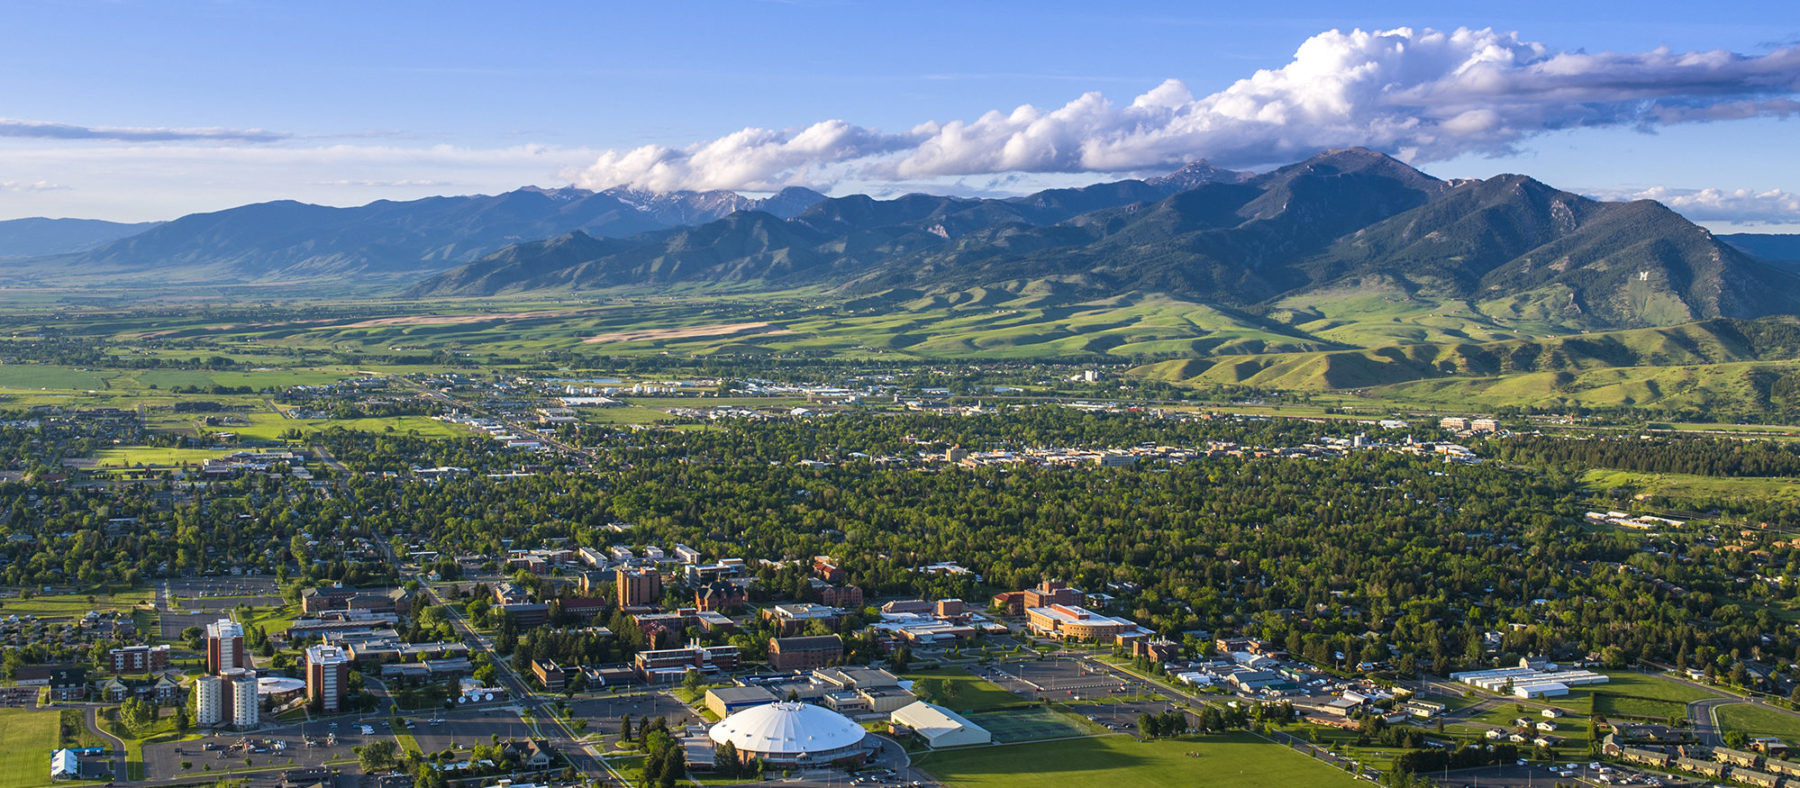
\includegraphics[width=5in,height=\textheight]{images/msu-campus.jpg}}
\usepackage{etoolbox}
\makeatletter
\providecommand{\subtitle}[1]{% add subtitle to \maketitle
  \apptocmd{\@title}{\par {\large #1 \par}}{}{}
}
\makeatother
\subtitle{Spring 2025\\
Montana State University}
\author{Melinda Yager\\
Jade Schmidt\\
Stacey Hancock}
\date{}

\begin{document}
\maketitle

\newpage
\thispagestyle{empty}

This resource was developed by Melinda Yager, Jade Schmidt, and Stacey Hancock in 2021 to accompany the online textbook: Hancock, S., Carnegie, N., Meyer, E., Schmidt, J., and Yager, M. (2021). \emph{Montana State Introductory Statistics with R}. Montana State University. \url{https://mtstateintrostats.github.io/IntroStatTextbook/}.

This resource is released under a \href{https://creativecommons.org/licenses/by-nc-sa/4.0/}{Creative Commons BY-NC-SA 4.0} license unless otherwise noted.

\setcounter{tocdepth}{1}
\addtocontents{toc}{\protect\thispagestyle{empty}}
\tableofcontents
\thispagestyle{empty}

\newpage
\setcounter{page}{1}

\chapter*{Preface}\label{preface}
\addcontentsline{toc}{chapter}{Preface}

This coursepack accompanies the textbook for STAT 216: Montana State Introductory Statistics with R, which can be found at \url{https://mtstateintrostats.github.io/IntroStatTextbook/}. The syllabus for the course (including the course calendar), data sets, and links to D2L Brightspace, Gradescope, and the MSU RStudio server can be found on the course webpage: \url{https://math.montana.edu/courses/s216/}.
Other notes and review materials are linked in D2L.

Each of the activities in this workbook is designed to target specific learning outcomes of the course, giving you practice with important statistical concepts in a group setting with instructor guidance. In addition to the in-class activities for the course, video notes are provided to aid in taking notes while you complete the required videos. Bring this workbook with you to class each class period, and take notes in the workbook as you would your own notes. A well-written completed workbook will provide an optimal study guide for exams!

All activities and labs in this coursepack will be completed during class time. Parts of each lab will be turned in on Gradescope. To aid in your understanding, read through the introduction for each activity before attending class each day.

STAT 216 is a 3-credit in-person course. In our experience, it takes six to nine hours per week outside of class to achieve a good grade in this class. By ``good'' we mean at least a C because a grade of D or below does not count toward fulfilling degree requirements. Many of you set your goals higher than just getting a C, and we fully support that. You need roughly nine hours per week to review past activities, read feedback on previous assignments, complete current assignments, and prepare for the next day's class. A typical week in the life of a STAT 216 student looks like:

\begin{itemize}
\tightlist
\item
  \emph{Prior to class meeting}:

  \begin{itemize}
  \tightlist
  \item
    Read assigned sections of the textbook, using the provided reading guides to take notes on the material.
  \item
    Watch the provided videos, taking notes in the coursepack.
  \item
    Read through the introduction to the day's in-class activity.
  \item
    Read through the week's homework assignment and note any questions you may have on the content.
  \end{itemize}
\item
  \emph{During class meeting}:

  \begin{itemize}
  \tightlist
  \item
    Work through the guided activity, in-class activity or weekly lab with your classmates and instructor, taking detailed notes on your answers to each question in the activity.
  \end{itemize}
\item
  \emph{After class meeting}:

  \begin{itemize}
  \tightlist
  \item
    Complete any parts of the activity you did not complete in class.
  \item
    Review the activity solutions in the Math and Stat Center, and take notes on key points.
  \item
    Complete any remaining assigned readings for the week.
  \item
    Complete the week's homework assignment.
  \end{itemize}
\end{itemize}

\nocite{*}

\chapter{Inference for a Quantitative Response with Independent Samples}\label{inference-for-a-quantitative-response-with-independent-samples}

\section{Vocabulary Review and Key Topics}\label{vocabulary-review-and-key-topics}

Review the Golden Ticket posted in the resources at the end of the coursepack for a summary of a categorical explanatory variable and a quantitative response variable for independent samples. Module 12 will cover both simulation and theory-based methods of inference.

Types of plot for independent variables

\begin{itemize}
\item
  \textbf{Side-by-side boxplots}: plots a boxplot of the five number summary for each categorical level
\item
  R code to create side-by-side boxplots:
\end{itemize}

\begin{Shaded}
\begin{Highlighting}[]
\NormalTok{object }\SpecialCharTok{\%\textgreater{}\%}  \CommentTok{\# Data set piped into...}
  \FunctionTok{ggplot}\NormalTok{(}\FunctionTok{aes}\NormalTok{(}\AttributeTok{y =}\NormalTok{ response, }\AttributeTok{x =}\NormalTok{ explanatory))}\SpecialCharTok{+}  \CommentTok{\# Identify variables}
  \FunctionTok{geom\_boxplot}\NormalTok{()}\SpecialCharTok{+}  \CommentTok{\# Tell it to make a box plot}
  \FunctionTok{labs}\NormalTok{(}\AttributeTok{title =} \StringTok{"Don\textquotesingle{}t forget to include a title"}\NormalTok{,  }\CommentTok{\# Title: should include the type of plot,}
       \CommentTok{\# observational units, variables}
       \AttributeTok{x =} \StringTok{"x{-}axis label"}\NormalTok{,    }\CommentTok{\# x{-}axis label}
       \AttributeTok{y =} \StringTok{"y{-}axis label"}\NormalTok{)  }\CommentTok{\# y{-}axis label}
\end{Highlighting}
\end{Shaded}

\begin{itemize}
\item
  \textbf{Stacked histogram}: plots one histogram for each level of the categorical variable
\item
  \textbf{Stacked dotplots}: plots one dotplot for each level of the categorical variable
\item
  Four characteristics to compare boxplots

  \begin{itemize}
  \item
    Shape (symmetric or skewed)
  \item
    Center
  \item
    Spread
  \item
    Outliers?
  \end{itemize}
\end{itemize}

Summary measure

\begin{itemize}
\item
  \textbf{Difference in mean}: measures the difference in mean values between the two categorical groups
\item
  Parameter notation for difference in means: \(\mu_1 - \mu_2\), where 1 represents the 1st group of the explanatory variable and 2 represents the 2nd group
\item
  Sample notation for difference in means: \(\bar{x}_1 - \bar{x}_2\)
\end{itemize}

\vspace{1mm}

\begin{itemize}
\item
  R code to find the summary statistics

  \begin{itemize}
  \tightlist
  \item
    Note: review the interpretations of the other summary measures from Module 6
  \end{itemize}
\end{itemize}

\begin{Shaded}
\begin{Highlighting}[]
\NormalTok{object }\SpecialCharTok{\%\textgreater{}\%}
  \FunctionTok{reframe}\NormalTok{(}\FunctionTok{favstats}\NormalTok{(response}\SpecialCharTok{\textasciitilde{}}\NormalTok{explantory))}
\end{Highlighting}
\end{Shaded}

\subsection*{Hypothesis Testing}\label{hypothesis-testing}
\addcontentsline{toc}{subsection}{Hypothesis Testing}

Hypotheses:

\[H_0: \mu_1 - \mu_2 = 0 ~ \text{or}~ H_0: \mu_1 = \mu_2 \]
\[H_A: \mu_1 - \mu_2 \left\{
\begin{array}{ll}
< \\
\ne \\
< \\
\end{array}
\right\}
0 
~ \text{or} ~ H_A:
\mu_1 \left\{
\begin{array}{ll}
< \\
\ne \\
< \\
\end{array}
\right\}
\mu_2 \]

\subsection*{Simulation Hypothesis Testing}\label{simulation-hypothesis-testing}
\addcontentsline{toc}{subsection}{Simulation Hypothesis Testing}

\begin{itemize}
\tightlist
\item
  R code for simulation methods to find the p-value using the \texttt{two\_mean\_test} function in the \texttt{catstats} package.
\end{itemize}

\begin{Shaded}
\begin{Highlighting}[]
\FunctionTok{two\_mean\_test}\NormalTok{(response}\SpecialCharTok{\textasciitilde{}}\NormalTok{explanatory, }\CommentTok{\#Enter the names of the variables }
               \AttributeTok{data =}\NormalTok{ object,  }\CommentTok{\# Enter the name of the dataset}
              \AttributeTok{first\_in\_subtraction =} \StringTok{"xx"}\NormalTok{, }\CommentTok{\# First outcome in order of subtraction }
               \AttributeTok{number\_repetitions =} \DecValTok{10000}\NormalTok{,  }\CommentTok{\# Number of simulations }
               \AttributeTok{as\_extreme\_as =} \SpecialCharTok{{-}}\NormalTok{xx,  }\CommentTok{\# Observed statistic }
               \AttributeTok{direction =} \StringTok{"xx"}\NormalTok{)  }\CommentTok{\# Direction of alternative: "greater", "less", or "two{-}sided"}
\end{Highlighting}
\end{Shaded}

\subsection*{Simulation Confidence Interval}\label{simulation-confidence-interval}
\addcontentsline{toc}{subsection}{Simulation Confidence Interval}

\begin{itemize}
\tightlist
\item
  R code to find the simulation confidence interval using the \texttt{twomean\_bootstrap\_CI} function from the \texttt{catstats} package.
\end{itemize}

\begin{Shaded}
\begin{Highlighting}[]
\FunctionTok{two\_mean\_bootstrap\_CI}\NormalTok{(response }\SpecialCharTok{\textasciitilde{}}\NormalTok{ explanatory, }\CommentTok{\#Enter the name of the variables}
                      \AttributeTok{data =}\NormalTok{ object,  }\CommentTok{\# Enter the name of the data set}
                      \AttributeTok{first\_in\_subtraction =} \StringTok{"xx"}\NormalTok{, }\CommentTok{\# First value in order of subtraction}
                      \AttributeTok{number\_repetitions =} \DecValTok{10000}\NormalTok{,  }\CommentTok{\# Number of simulations}
                      \AttributeTok{confidence\_level =}\NormalTok{ xx)}
\end{Highlighting}
\end{Shaded}

\begin{itemize}
\tightlist
\item
  Review how to interpret the confidence interval for two groups from Module 8
\end{itemize}

\subsection*{Theory-based methods}\label{theory-based-methods}
\addcontentsline{toc}{subsection}{Theory-based methods}

\begin{itemize}
\item
  \textbf{Conditions for the sampling distribution of \(\bar{x}_1 - \bar{x}_2\) to follow an approximate normal distribution}:

  \begin{itemize}
  \item
    \textbf{Independence}: The sample's observations are independent, e.g., are from a simple random sample and there is independence between groups. (\emph{Remember}: This also must be true to use simulation methods!)
  \item
    \textbf{Normality Condition}: Either the sample observations come from a normally distributed population or we have a large enough sample size. When we have two samples, we need to check this condition for each group! To check this condition, use the following rules of thumb (for both \(n_1\) and \(n_2\)):

    \begin{itemize}
    \item
      \(n < 30\): The distribution of the sample must be approximately normal with no outliers.
    \item
      \(30 \le n < 100\): We can relax the condition a little; the distribution of the sample must have no extreme outliers or skewness.
    \item
      \(n \ge 100\): Can assume the sampling distribution of \(\bar{x}\) is nearly normal, even if the underlying distribution of individual observations is not.
    \end{itemize}
  \end{itemize}
\item
  \textbf{t-distribution}: a theoretical distribution that is symmetric with a given degrees of freedom smallest sample size minus 1 (\(n-1\))
\end{itemize}

\[t_{n-1}\]

\begin{itemize}
\tightlist
\item
  Calculation of standard error:
\end{itemize}

\[SE(\bar{x}_1 - \bar{x}_2) = \sqrt{\frac{{s_1}^2}{n_1}+\frac{{s_2}^2}{n_2}}\]

\begin{itemize}
\tightlist
\item
  Calculation of the standardized difference in sample mean:
\end{itemize}

\[t = \frac{\bar{x}_1-\bar{x}_2-0}{SE(\bar{x}_1 - \bar{x}_2)}\]

\begin{itemize}
\item
  The p-value can be found by using the pt function.

  \begin{itemize}
  \item
    Enter the value of the standardized statistic for xx
  \item
    Enter the df smallest \((n-1)\) for yy
  \item
    If a greater than alternative, change lower.tail = TRUE to FALSE.
  \item
    If a two-sided test, multiply by 2.
  \end{itemize}
\end{itemize}

\begin{Shaded}
\begin{Highlighting}[]
\FunctionTok{pt}\NormalTok{(xx, }\AttributeTok{df =}\NormalTok{ yy, }\AttributeTok{lower.tail=}\ConstantTok{TRUE}\NormalTok{)}
\end{Highlighting}
\end{Shaded}

\subsection*{Theory-based methods to find the confidence interval}\label{theory-based-methods-to-find-the-confidence-interval}
\addcontentsline{toc}{subsection}{Theory-based methods to find the confidence interval}

\begin{itemize}
\tightlist
\item
  Calculation of the confidence interval for a difference in sample means
\end{itemize}

\[\bar{x}_1-\bar{x}_2\pm t^*\times SE(\bar{x}_1-\bar{x}_2)\]

\begin{itemize}
\item
  R code to find the multiplier for the confidence interval using theory-based methods.

  \begin{itemize}
  \item
    qt will give you the multiplier using the t-distribution with smallest \(n-1\) df (enter for yy)
  \item
    Enter the percentile for the given confidence level
  \end{itemize}
\end{itemize}

\begin{Shaded}
\begin{Highlighting}[]
\FunctionTok{qt}\NormalTok{(percentile, }\AttributeTok{df=}\NormalTok{yy, }\AttributeTok{lower.tail=}\ConstantTok{FALSE}\NormalTok{)}
\end{Highlighting}
\end{Shaded}

\newpage

\section{Video Notes: Inference for Independent Samples}\label{video-notes-inference-for-independent-samples}

Read Chapters 19 and 20 in the course textbook. Use the following videos to complete the video notes for Module 10.

\subsection{Course Videos}\label{course-videos}

\begin{itemize}
\item
  19.1
\item
  19.2
\item
  19.3TheoryTests
\item
  19.4TheoryInterval
\end{itemize}

\setstretch{1}

\subsection*{Single categorical, single quantitative variable with independent samples}\label{single-categorical-single-quantitative-variable-with-independent-samples}
\addcontentsline{toc}{subsection}{Single categorical, single quantitative variable with independent samples}

\setstretch{1.5}

\begin{itemize}
\item
  In this module, we will study inference for a \_\_\_\_\_\_\_\_\_\_\_\_\_\_\_\_\_\_\_\_\_\_ explanatory variable and a \_\_\_\_\_\_\_\_\_\_\_\_\_\_\_\_\_\_\_\_\_\_\_\_\_ response variable where the two groups are \_\_\_\_\_\_\_\_\_\_\_\_\_\_\_\_\_\_\_\_\_\_\_\_\_\_\_\_.
\item
  Independent groups: When the measurements in one sample are not
  related to the measurements in the other sample.
\end{itemize}

\setstretch{1}

\begin{itemize}
\item
  Two random samples taken separately from two populations and the same response variable is recorded. Compare the average number of sick days off from work for people who had a flu shot and people who didn't.
\item
  Participants are randomly assigned to one of two treatment conditions, and the same response variable is recorded.
\end{itemize}

Rather than analyzing the differences as a single mean we will calculate summary statistics on each sample.

Example: Fifty-one (51) college students volunteered to look at impacts on memorization, specifically if putting letters into recognizable patterns (like FBI, CIA, EDA, CDC, etc.) would increase the number letters memorized. (Miller 1956) The college students were randomly assigned to either a recognizable or non-recognizable letter group. After a period of study time, the number of letters memorized was collected on each study. Is there evidence that putting letters into recognizable letter groups improve memory?

\setstretch{1.5}

\begin{itemize}
\tightlist
\item
  The summary measure for two independent groups is the \_\_\_\_\_\_\_\_\_\_\_\_\_\_\_\_\_\_\_\_\_\_ in \_\_\_\_\_\_\_\_\_\_\_\_\_\_\_\_\_\_\_\_\_\_\_\_\_\_\_\_\_.
\end{itemize}

\setstretch{1}

\setstretch{1.5}

Notation for Independent Groups

\begin{itemize}
\item
  Population mean for group 1:
\item
  Population mean for group 2:
\item
  Sample mean for group 1:
\item
  Sample mean for group 2:
\item
  Sample difference in means:
\item
  Population standard deviation for group 1:
\item
  Population standard deviation for group 2:
\item
  Sample standard deviation for group 1:
\item
  Sample standard deviation for group 2:
\item
  Sample size for group 1:
\item
  Sample size for group 2:
\end{itemize}

\setstretch{1}

Why should we treat this as two independent groups rather than paired data?

\vspace{0.6in}

\subsection*{Hypothesis Testing}\label{hypothesis-testing-1}
\addcontentsline{toc}{subsection}{Hypothesis Testing}

Conditions:

\begin{itemize}
\tightlist
\item
  Independence: the response for one observational unit will not influence the outcome for another observational unit
\end{itemize}

Null hypothesis assumes ``no effect'', ``no difference'', ``nothing interesting happening'', etc.

\rgi Always of form: ``parameter'' = null value

\(H_0:\)

\vspace{0.5in}

\(H_A:\)

\vspace{0.5in}

\begin{itemize}
\tightlist
\item
  Research question determines the alternative hypothesis.
\end{itemize}

Write the null and alternative hypotheses for the letters study:

In notation:

\(H_0:\)

\vspace{0.2in}

\(H_A:\)

\vspace{0.2in}

\begin{Shaded}
\begin{Highlighting}[]
\NormalTok{letters}\OtherTok{\textless{}{-}}\FunctionTok{read.csv}\NormalTok{(}\StringTok{"data/letters.csv"}\NormalTok{)}
\NormalTok{letters }\SpecialCharTok{\%\textgreater{}\%}
    \FunctionTok{reframe}\NormalTok{(}\FunctionTok{favstats}\NormalTok{(Memorized}\SpecialCharTok{\textasciitilde{}}\NormalTok{Grouped))}
\end{Highlighting}
\end{Shaded}

\begin{verbatim}
#>           Grouped min Q1 median    Q3 max     mean       sd  n missing
#> 1 NotRecognizable   1  6     12 14.75  24 11.15385 6.576883 26       0
#> 2    Recognizable   1  6     15 21.00  30 14.32000 8.518216 25       0
\end{verbatim}

Summary statistic:

\vspace{0.4in}

Interpret the summary statistic in context of the problem:

\vspace{0.4in}

\begin{Shaded}
\begin{Highlighting}[]
\NormalTok{letters}\SpecialCharTok{\%\textgreater{}\%}
  \FunctionTok{ggplot}\NormalTok{(}\FunctionTok{aes}\NormalTok{(}\AttributeTok{y =}\NormalTok{ Memorized, }\AttributeTok{x =}\NormalTok{ Grouped))  }\SpecialCharTok{+} \CommentTok{\#Enter the name of the explanatory and response variable}
  \FunctionTok{geom\_boxplot}\NormalTok{()}\SpecialCharTok{+}
  \FunctionTok{labs}\NormalTok{(}\AttributeTok{title =} \StringTok{"Boxplot of Number of Letters memorized by Type }
\StringTok{       of Grouping for College Students"}\NormalTok{, }\CommentTok{\#Title your plot}
       \AttributeTok{y =} \StringTok{"Number of letters memorized"}\NormalTok{, }\CommentTok{\#y{-}axis label}
       \AttributeTok{x =} \StringTok{"Letter Grouping"}\NormalTok{) }\CommentTok{\#x{-}axis label}
\end{Highlighting}
\end{Shaded}

\begin{center}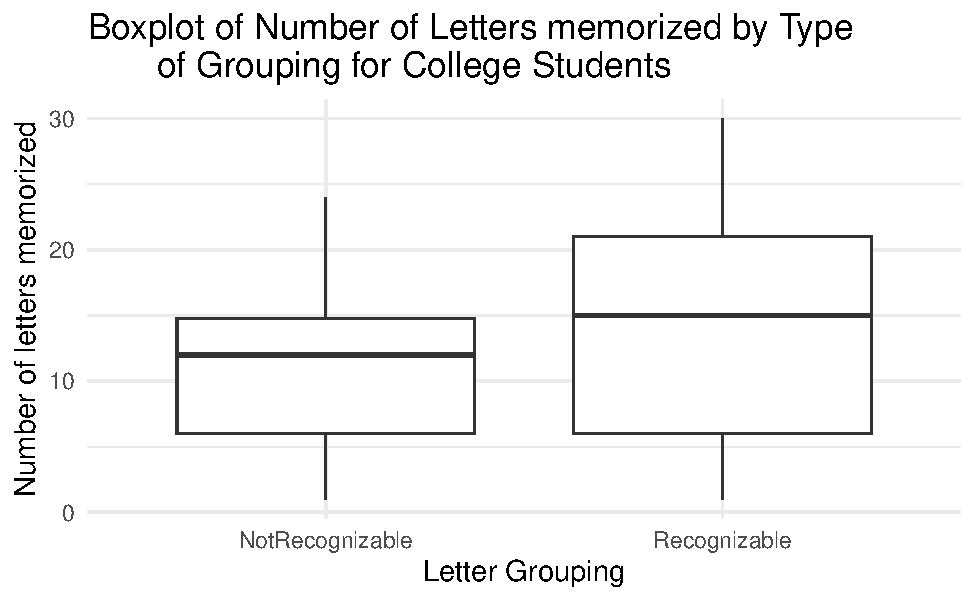
\includegraphics[width=0.6\linewidth]{12-VN12-1ofeach_files/figure-latex/unnamed-chunk-2-1} \end{center}

\subsubsection*{Simulation-based method}\label{simulation-based-method}
\addcontentsline{toc}{subsubsection}{Simulation-based method}

\begin{itemize}
\item
  Simulate many samples assuming \(H_0: \mu_1 = \mu_2\)

  \begin{itemize}
  \item
    Write the response variable values on cards
  \item
    Mix the explanatory variable groups together
  \item
    Shuffle cards into two explanatory variable groups to represent the sample size in each group (\(n_1\) and \(n_2\))
  \item
    Calculate and plot the simulated difference in sample means from each simulation
  \item
    Repeat 1000 times (simulations) to create the null distribution
  \item
    Find the proportion of simulations at least as extreme as \(\bar{x}_1 - \bar{x}_2\)
  \end{itemize}
\end{itemize}

\vspace{1mm}

\begin{Shaded}
\begin{Highlighting}[]
\FunctionTok{set.seed}\NormalTok{(}\DecValTok{216}\NormalTok{)}
\FunctionTok{two\_mean\_test}\NormalTok{(Memorized}\SpecialCharTok{\textasciitilde{}}\NormalTok{Grouped, }\CommentTok{\#Enter the names of the variables}
              \AttributeTok{data =}\NormalTok{ letters,  }\CommentTok{\# Enter the name of the dataset}
              \AttributeTok{first\_in\_subtraction =} \StringTok{"Recognizable"}\NormalTok{, }\CommentTok{\# First outcome in order of subtraction}
              \AttributeTok{number\_repetitions =} \DecValTok{10000}\NormalTok{,  }\CommentTok{\# Number of simulations}
              \AttributeTok{as\_extreme\_as =} \FloatTok{3.166}\NormalTok{,  }\CommentTok{\# Observed statistic}
              \AttributeTok{direction =} \StringTok{"greater"}\NormalTok{)  }\CommentTok{\# Direction of alternative: "greater", "less", or "two{-}sided"}
\end{Highlighting}
\end{Shaded}

\begin{center}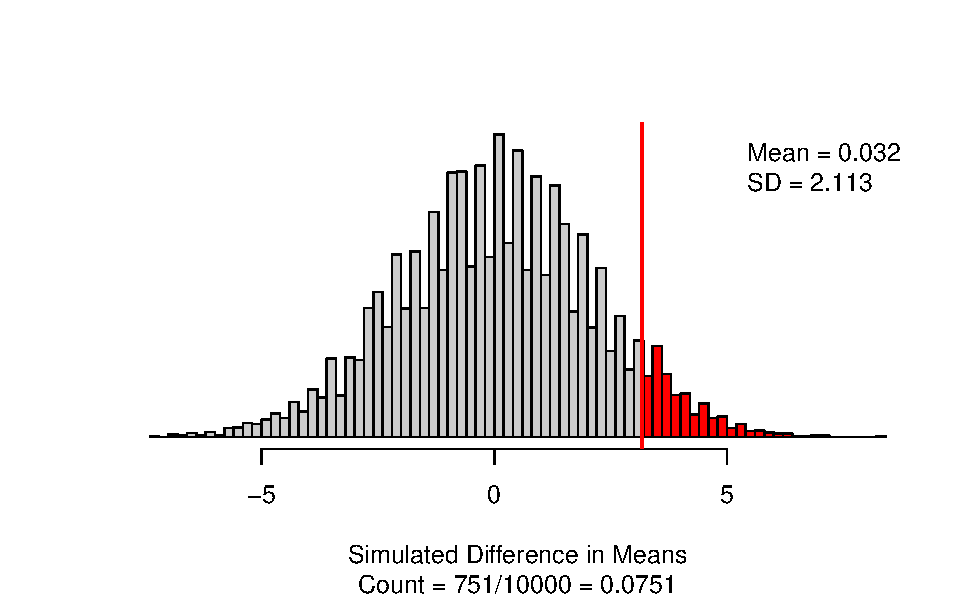
\includegraphics[width=0.7\linewidth]{12-VN12-1ofeach_files/figure-latex/unnamed-chunk-3-1} \end{center}

Explain why the null distribution is centered at the value of zero:

\vspace{0.8in}

Interpretation of the p-value:

\begin{itemize}
\item
  Statement about probability or proportion of samples
\item
  Statistic (summary measure and value)
\item
  Direction of the alternative
\item
  Null hypothesis (in context)
\end{itemize}

\vspace{0.8in}

Conclusion:

\begin{itemize}
\item
  Amount of evidence
\item
  Parameter of interest
\item
  Direction of the alternative hypothesis
\end{itemize}

\vspace{0.6in}

\newpage

\subsection*{Confidence interval}\label{confidence-interval}
\addcontentsline{toc}{subsection}{Confidence interval}

To estimate the difference in true mean we will create a confidence interval.

\subsubsection*{Simulation-based method - Video 19.2}\label{simulation-based-method---video-19.2}
\addcontentsline{toc}{subsubsection}{Simulation-based method - Video 19.2}

\begin{itemize}
\item
  Write the response variable values on cards
\item
  Keep explanatory variable groups separate
\item
  Sample with replacement \(n_1\) times in explanatory variable group 1 and \(n_2\) times in explanatory variable group 2
\item
  Calculate and plot the simulated difference in sample means from each simulation
\item
  Repeat 1000 times (simulations) to create the bootstrap distribution
\item
  Find the cut-offs for the middle X\% (confidence level) in a bootstrap distribution.
\end{itemize}

For the letters example, we will estimate the difference in true mean number of letters recognized for students given recognizable letter groupings and students given non-recognizable letter groupings.

\begin{Shaded}
\begin{Highlighting}[]
\FunctionTok{set.seed}\NormalTok{(}\DecValTok{216}\NormalTok{)}
\FunctionTok{two\_mean\_bootstrap\_CI}\NormalTok{(Memorized }\SpecialCharTok{\textasciitilde{}}\NormalTok{ Grouped, }\CommentTok{\#Enter the name of the variables}
                      \AttributeTok{data =}\NormalTok{ letters,  }\CommentTok{\# Enter the name of the data set}
                      \AttributeTok{first\_in\_subtraction =} \StringTok{"Recognizable"}\NormalTok{, }\CommentTok{\# First value in order of subtraction}
                      \AttributeTok{number\_repetitions =} \DecValTok{10000}\NormalTok{,  }\CommentTok{\# Number of simulations}
                      \AttributeTok{confidence\_level =} \FloatTok{0.95}\NormalTok{)}
\end{Highlighting}
\end{Shaded}

\begin{center}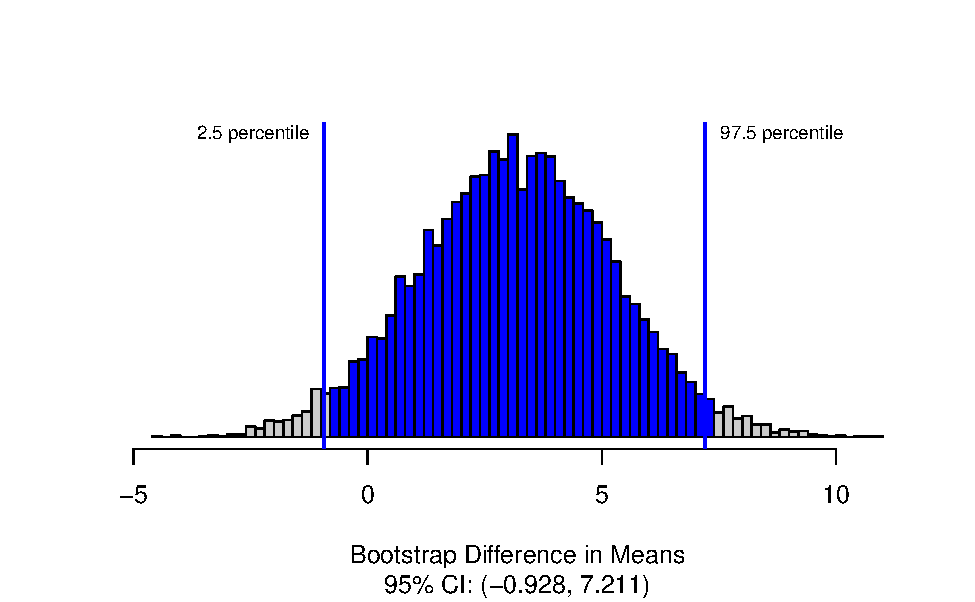
\includegraphics[width=0.7\linewidth]{12-VN12-1ofeach_files/figure-latex/unnamed-chunk-4-1} \end{center}

Confidence interval interpretation:

\begin{itemize}
\item
  How confident you are (e.g., 90\%, 95\%, 98\%, 99\%)
\item
  Parameter of interest
\item
  Calculated interval
\item
  Order of subtraction when comparing two groups
\end{itemize}

\vspace{0.8in}

\subsubsection*{Theory-based method - Video 19.3TheoryTests}\label{theory-based-method---video-19.3theorytests}
\addcontentsline{toc}{subsubsection}{Theory-based method - Video 19.3TheoryTests}

Example: Every year, orange and black monarch butterflies migrate from their summer breeding grounds in the US and Canada to mountain forests in central Mexico, where they hibernate for the winter. Due to abnormal weather patterns and drought affecting monarch habitats and feeding grounds, the population of monarch butterflies is estimated to have decreased by 53\% from the 2018-2019 wintering season to the 2019-2020 wintering season (WWF, 2020). While conservationists often resort to captive-rearing with the goal of raising biologically indistinct individuals for release into the wild, tagging studies have shown that captive-reared monarchs have lower migratory success compared to wild monarchs. For this study, the researchers raised 67 monarchs (descended from wild monarchs) from eggs to maturity and then compared them to a group of 40 wild-caught monarchs. The researchers want to explore whether the maximum grip strength (how many Newtons a butterfly exerts at the moment of release when gently tugged from a mesh-covered perch) differs between captive-reared and wild-caught monarchs. Use Captive -- Wild for order of subtraction.

Write the null and alternative hypotheses in notation.

\(H_0:\)

\vspace{0.2in}

\(H_A:\)

\vspace{0.2in}

\begin{Shaded}
\begin{Highlighting}[]
\NormalTok{butterfly }\OtherTok{\textless{}{-}}\FunctionTok{read.csv}\NormalTok{(}\StringTok{"data/butterfly1.csv"}\NormalTok{)}

\NormalTok{butterflies }\OtherTok{\textless{}{-}}\NormalTok{ butterfly }\SpecialCharTok{\%\textgreater{}\%} \FunctionTok{na.omit}\NormalTok{() }\SpecialCharTok{\%\textgreater{}\%}
    \FunctionTok{rename}\NormalTok{(}\AttributeTok{Monarch\_Group =} \StringTok{"Monarch.Group"}\NormalTok{,}
           \AttributeTok{MaxGrip =} \StringTok{"Max.Grip.Strength..N."}\NormalTok{) }\SpecialCharTok{\%\textgreater{}\%}
    \FunctionTok{mutate}\NormalTok{(}\AttributeTok{Monarch\_Group =} \FunctionTok{factor}\NormalTok{(Monarch\_Group),}
           \AttributeTok{Sex =} \FunctionTok{factor}\NormalTok{(Sex)) }\SpecialCharTok{\%\textgreater{}\%}
    \FunctionTok{mutate}\NormalTok{(}\AttributeTok{Monarch\_Group =} \FunctionTok{fct\_collapse}\NormalTok{(Monarch\_Group,}\StringTok{"Captive"} \OtherTok{=} \FunctionTok{c}\NormalTok{(}\StringTok{"Incubator {-} Fall conditions"}\NormalTok{, }\StringTok{"Rearing room {-} summer conditions"}\NormalTok{), }\StringTok{"Wild"} \OtherTok{=} \StringTok{"Wild migrants"}\NormalTok{))}

\NormalTok{butterflies }\SpecialCharTok{\%\textgreater{}\%}
    \FunctionTok{reframe}\NormalTok{(}\FunctionTok{favstats}\NormalTok{(MaxGrip}\SpecialCharTok{\textasciitilde{}}\NormalTok{Monarch\_Group))}
\end{Highlighting}
\end{Shaded}

\begin{verbatim}
#>   Monarch_Group   min    Q1 median     Q3   max      mean         sd  n missing
#> 1       Captive 0.081 0.162  0.217 0.2845 0.596 0.2363731 0.09412948 67       0
#> 2          Wild 0.108 0.271  0.352 0.4330 0.650 0.3607500 0.14066796 40       0
\end{verbatim}

\begin{center}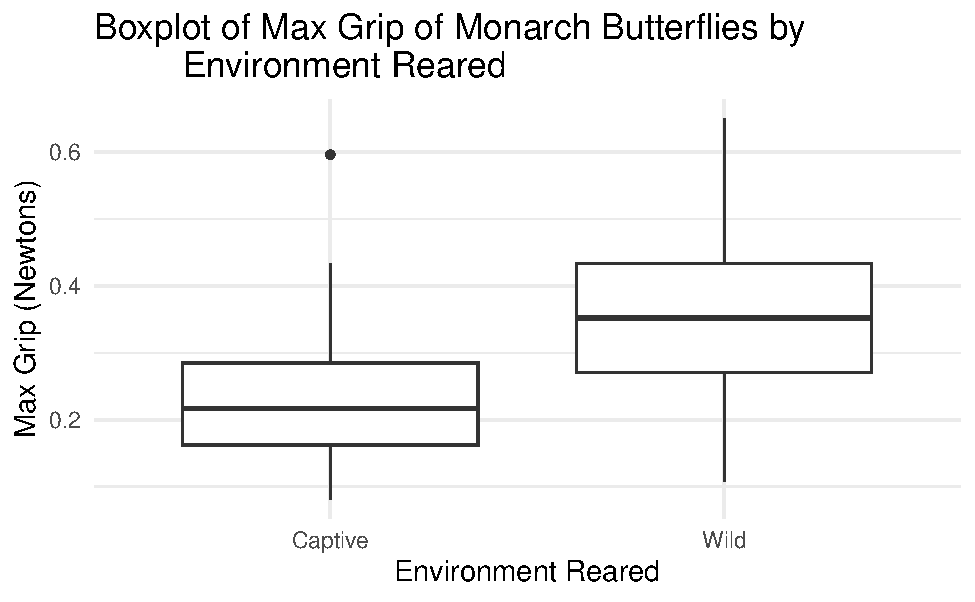
\includegraphics[width=0.7\linewidth]{12-VN12-1ofeach_files/figure-latex/unnamed-chunk-6-1} \end{center}

Conditions:

\begin{itemize}
\item
  Independence: the response for one observational unit will not influence the outcome for another observational unit
\item
  Large enough sample size
\end{itemize}

\vspace{1in}

Like with paired data the t-distribution can be used to model the difference in means.

\setstretch{1.5}

\begin{itemize}
\tightlist
\item
  For independent samples we use the \_\_\_\_\_\_- distribution
  with \_\_\_\_\_\_\_\_\_\_\_\_\_\_\_\_ degrees of freedom to approximate the sampling distribution.
\end{itemize}

\setstretch{1}

Theory-based test:

\begin{itemize}
\item
  Calculate the standardized statistic
\item
  Find the area under the t-distribution with the smallest \(n - 1\) df {[}min(\(n_1-1, n_2-1\)){]} at least as extreme as the standardized statistic
\end{itemize}

Equation for the standard error of the difference in sample mean:

\vspace{0.5in}

Equation for the standardized difference in sample mean:

\vspace{0.5in}

Are the conditions met to analyze the butterfly data using theory based-methods?

\vspace{0.8in}

Calculate the standardized difference in mean max grip strength.

\begin{itemize}
\tightlist
\item
  First calculate the \(SE(\bar{x}_1 - \bar{x}_2)\)
\end{itemize}

\vspace{0.6in}

\begin{itemize}
\tightlist
\item
  Then calculate the T-score
\end{itemize}

\vspace{1in}

What theoretical distribution should we use to find the p-value?

\vspace{0.3in}

To find the theory-based p-value:

\begin{Shaded}
\begin{Highlighting}[]
\FunctionTok{pt}\NormalTok{(}\SpecialCharTok{{-}}\DecValTok{5}\NormalTok{, }\AttributeTok{df=}\DecValTok{39}\NormalTok{, }\AttributeTok{lower.tail=}\ConstantTok{FALSE}\NormalTok{)}\SpecialCharTok{*}\DecValTok{2}
\end{Highlighting}
\end{Shaded}

\begin{verbatim}
#> [1] 1.999987
\end{verbatim}

Conclusion:

\begin{itemize}
\item
  Amount of evidence
\item
  Parameter of interest
\item
  Direction of the alternative hypothesis
\end{itemize}

\vspace{0.6in}

\subsubsection*{Confidence Interval - Video 19.3TheoryIntervals}\label{confidence-interval---video-19.3theoryintervals}
\addcontentsline{toc}{subsubsection}{Confidence Interval - Video 19.3TheoryIntervals}

\begin{itemize}
\tightlist
\item
  Calculate the interval centered at the sample statistic
\end{itemize}

\rgi \(\text{statistic} \pm \text{margin of error}\)

\vspace{0.8in}

Using the butterfly data, calculate the 99\% confidence interval.

\begin{Shaded}
\begin{Highlighting}[]
\NormalTok{butterflies }\SpecialCharTok{\%\textgreater{}\%}
    \FunctionTok{reframe}\NormalTok{(}\FunctionTok{favstats}\NormalTok{(MaxGrip}\SpecialCharTok{\textasciitilde{}}\NormalTok{Monarch\_Group))}
\end{Highlighting}
\end{Shaded}

\begin{verbatim}
#>   Monarch_Group   min    Q1 median     Q3   max      mean         sd  n missing
#> 1       Captive 0.081 0.162  0.217 0.2845 0.596 0.2363731 0.09412948 67       0
#> 2          Wild 0.108 0.271  0.352 0.4330 0.650 0.3607500 0.14066796 40       0
\end{verbatim}

\begin{itemize}
\tightlist
\item
  Need the \(t^*\) multiplier for a 99\% confidence interval from a t-distribution with \_\_\_\_\_\_\_\_\_ df.
\end{itemize}

\begin{Shaded}
\begin{Highlighting}[]
\FunctionTok{qt}\NormalTok{(}\FloatTok{0.995}\NormalTok{, }\AttributeTok{df=}\DecValTok{39}\NormalTok{, }\AttributeTok{lower.tail =} \ConstantTok{TRUE}\NormalTok{)}
\end{Highlighting}
\end{Shaded}

\begin{verbatim}
#> [1] 2.707913
\end{verbatim}

\begin{itemize}
\tightlist
\item
  We will use the same value for the \(SE(\bar{x}_1-\bar{x}_2)\) as calculated for the standardized statistic.
\end{itemize}

\vspace{1in}

Calculate the margin of error for a 99\% confidence interval for the parameter of interest.

\vspace{0.5in}

Calculate a 99\% confidence interval for the parameter of interest.

\vspace{0.6in}

\subsection{Concept Check}\label{concept-check}

Be prepared for group discussion in the next class. One member from the table should write the answers to the following on the whiteboard.

\begin{enumerate}
\def\labelenumi{\arabic{enumi}.}
\tightlist
\item
  Why is the recognizable letter study analyzed as two independent groups rather than paired data?
\end{enumerate}

\vspace{0.6in}

\begin{enumerate}
\def\labelenumi{\arabic{enumi}.}
\setcounter{enumi}{1}
\tightlist
\item
  Write out the equation for the standard error for a difference in sample means.
\end{enumerate}

\vspace{1in}

\newpage

\section{Activity 24: Does behavior impact performance?}\label{activity-24-does-behavior-impact-performance}

\setstretch{1}

\subsection{Learning outcomes}\label{learning-outcomes}

\begin{itemize}
\item
  Create a side-by-side boxplot of one categorical explanatory variable and one quantitative response variable
\item
  Given a research question involving one categorical explanatory variable and one quantitative response variable, construct the null and alternative hypotheses
  in words and using appropriate statistical symbols.
\item
  Describe and perform a simulation-based hypothesis test for a difference in means.
\item
  Interpret and evaluate a p-value for a simulation-based hypothesis test for a difference in means.
\item
  Use bootstrapping to find a confidence interval for a difference in means.
\item
  Interpret a confidence interval for a difference in means.
\item
  Use a confidence interval to determine the conclusion of a hypothesis test.
\end{itemize}

\subsection{Terminology review}\label{terminology-review}

In today's activity, we will use simulation-based methods to analyze the association between one categorical explanatory variable and one quantitative response variable, where the groups formed by the categorical variable are independent. Some terms covered in this activity are:

\begin{itemize}
\item
  Independent groups
\item
  Difference in means
\end{itemize}

To review these concepts, see Chapter 19 in the textbook.

\subsection{Behavior and Performance}\label{behavior-and-performance}

A study in the Academy of Management Journal (Porath 2017) investigated how rude behaviors influence a victim's task performance. Randomly selected college students enrolled in a management course were randomly assigned to one of two experimental conditions: rudeness condition (45 students) and control group (53 students). Each student was asked to write down as many uses for a brick as possible in five minutes; this value (total number of uses) was used as a performance measure for each student, where higher values indicate better performance. During this time another individual showed up late for class. For those students in the rudeness condition, the facilitator displayed rudeness by berating the students in general for being irresponsible and unprofessional (due to the late-arriving person). No comments were made about the late-arriving person for students in the control group. Is there evidence that the average performance score for students in the rudeness condition is lower than for students in the control group? Use the order of subtraction of rudeness -- control.

\begin{itemize}
\item
  Download the R script file from D2L and upload to the RStudio server
\item
  Highlight and run lines 1--7
\end{itemize}

\begin{Shaded}
\begin{Highlighting}[]
\CommentTok{\# Read in data set}
\NormalTok{rude }\OtherTok{\textless{}{-}} \FunctionTok{read.csv}\NormalTok{(}\StringTok{"https://math.montana.edu/courses/s216/data/rude.csv"}\NormalTok{)}
\end{Highlighting}
\end{Shaded}

\newpage

\begin{itemize}
\tightlist
\item
  Highlight and run lines 11--19
\end{itemize}

\begin{Shaded}
\begin{Highlighting}[]
\CommentTok{\# Side{-}by{-}side box plots}
\NormalTok{rude }\SpecialCharTok{\%\textgreater{}\%}
\FunctionTok{ggplot}\NormalTok{(}\FunctionTok{aes}\NormalTok{(}\AttributeTok{x =}\NormalTok{ condition, }\AttributeTok{y =}\NormalTok{ number\_of\_uses)) }\SpecialCharTok{+}
    \FunctionTok{geom\_boxplot}\NormalTok{() }\SpecialCharTok{+} 
    \FunctionTok{labs}\NormalTok{(}\AttributeTok{title =} \StringTok{"Number of Uses for a Brick based on Behavior Condition}
\StringTok{         for College Students in a Management Course"}\NormalTok{,}
         \AttributeTok{x =} \StringTok{"Behavior"}\NormalTok{) }
\CommentTok{\# Summary statistics}
\NormalTok{rude }\SpecialCharTok{\%\textgreater{}\%} 
     \FunctionTok{reframe}\NormalTok{(}\FunctionTok{favstats}\NormalTok{(number\_of\_uses }\SpecialCharTok{\textasciitilde{}}\NormalTok{ condition))}
\CommentTok{\#\textgreater{}   condition min Q1 median Q3 max      mean       sd  n missing}
\CommentTok{\#\textgreater{} 1   control   0  6     12 17  30 11.811321 7.382559 53       0}
\CommentTok{\#\textgreater{} 2  rudeness   0  6      9 11  18  8.511111 3.992164 45       0}
\end{Highlighting}
\end{Shaded}

\begin{center}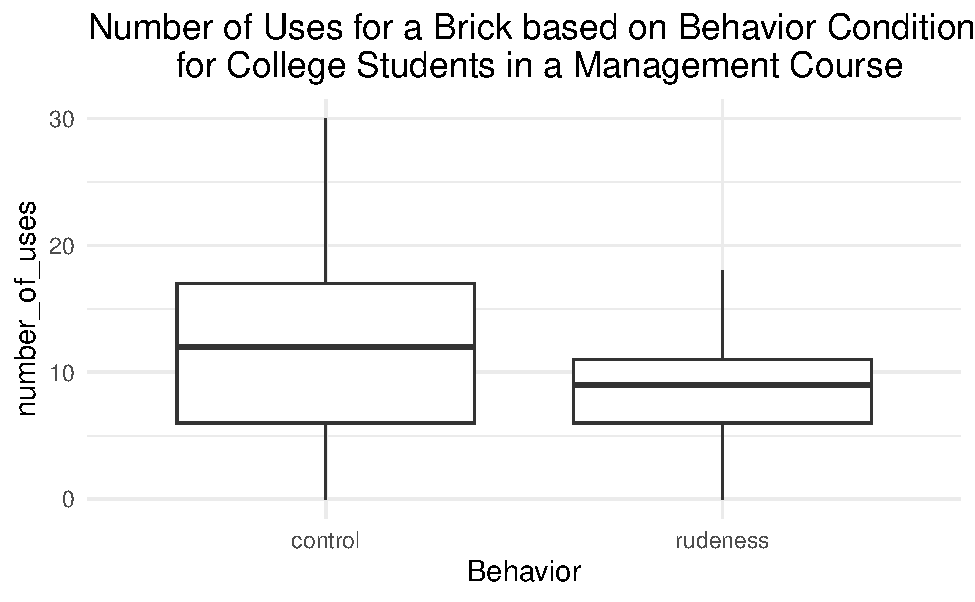
\includegraphics[width=0.6\linewidth]{12-A24-inference-1ofeach-simulation_files/figure-latex/unnamed-chunk-2-1} \end{center}

\subsubsection*{Quantitative variables review}\label{quantitative-variables-review}
\addcontentsline{toc}{subsubsection}{Quantitative variables review}

\begin{enumerate}
\def\labelenumi{\arabic{enumi}.}
\item
  Compare the distributions of the number of bricks between the two treatment conditions.

  \begin{itemize}
  \item
    What is the shape of each group?
    \vspace{0.3in}
  \item
    Which group has the higher center?
    \vspace{0.3in}
  \item
    What group has the larger spread?
    \vspace{0.3in}
  \item
    Does either distribution have outliers?
    \vspace{.3in}
  \end{itemize}
\item
  Is this an experiment or an observational study? Justify your answer.
\end{enumerate}

\vspace{1in}

\begin{enumerate}
\def\labelenumi{\arabic{enumi}.}
\setcounter{enumi}{2}
\tightlist
\item
  Explain why this is two independent samples and not paired data.
  \vspace{1in}
\end{enumerate}

\subsubsection*{Ask a research question}\label{ask-a-research-question}
\addcontentsline{toc}{subsubsection}{Ask a research question}

In this study we are assessing the difference in true mean number of uses for a brick given by college students enrolled in a management course assigned to a rudeness condition and for those assigned to a control group.

\begin{enumerate}
\def\labelenumi{\arabic{enumi}.}
\setcounter{enumi}{3}
\tightlist
\item
  What assumption are we making about the difference in true mean?
\end{enumerate}

\vspace{0.8in}

\begin{enumerate}
\def\labelenumi{\arabic{enumi}.}
\setcounter{enumi}{4}
\tightlist
\item
  Write the alternative hypothesis in notation.
\end{enumerate}

\vspace{0.5in}

\subsubsection*{Numerically Summarize the data}\label{numerically-summarize-the-data}
\addcontentsline{toc}{subsubsection}{Numerically Summarize the data}

\begin{enumerate}
\def\labelenumi{\arabic{enumi}.}
\setcounter{enumi}{5}
\tightlist
\item
  Calculate the summary statistic of interest (difference in means). What is the appropriate notation for this statistic?
\end{enumerate}

\vspace{0.5in}

Interpret this calculated value.

\vspace{0.6in}

\begin{enumerate}
\def\labelenumi{\arabic{enumi}.}
\setcounter{enumi}{6}
\item
  Write out the parameter of interest for this study in context of the study.

  \begin{itemize}
  \item
    To write in context:

    \begin{itemize}
    \item
      Population word (true, long-run, population)
    \item
      Summary measure (depends on the type of data)
    \item
      Context

      \begin{itemize}
      \item
        Observational units
      \item
        Variable(s)
        \vspace{1in}
      \end{itemize}
    \end{itemize}
  \end{itemize}
\end{enumerate}

In this study we are assessing the difference in true mean number of uses for a brick given by college students enrolled in a management course assigned to a rudeness condition and for those assigned to a control group.

\subsubsection*{Use statistical inferential methods to draw inferences from the data}\label{use-statistical-inferential-methods-to-draw-inferences-from-the-data}
\addcontentsline{toc}{subsubsection}{Use statistical inferential methods to draw inferences from the data}

\paragraph*{Hypothesis test}\label{hypothesis-test}
\addcontentsline{toc}{paragraph}{Hypothesis test}

Remember that the null distribution is created based on the assumption the null hypothesis is true. In this study, the null hypothesis states that there is no association between the two variables. This means that the values observed in the data set would have been the same regardless of the behavior condition.

To demonstrate this simulation, we could create cards to simulate a sample.

\begin{itemize}
\item
  Write the number of uses for a brick given by each student on one card.
\item
  Mix together and shuffle into two piles, one with 45 cards to represent the rudeness condition and one with 53 cards to represent the control group.
\item
  Calculate the difference in mean number of uses for a brick (rudeness - control)
\end{itemize}

We will use the \texttt{two\_mean\_test()} function in R (in the \texttt{catstats} package) to simulate the null distribution of differences in sample means and compute a p-value.

\begin{itemize}
\item
  Fill in the response and explanatory variable names
\item
  Fill in the missing values/names for the xx's in the R script file
\item
  Highlight and run lines 25--30
\end{itemize}

\begin{Shaded}
\begin{Highlighting}[]
\FunctionTok{set.seed}\NormalTok{(}\DecValTok{216}\NormalTok{)}
\FunctionTok{two\_mean\_test}\NormalTok{(response}\SpecialCharTok{\textasciitilde{}}\NormalTok{explanatory, }\CommentTok{\#Enter the names of the variables}
              \AttributeTok{data =}\NormalTok{ rude,  }\CommentTok{\# Enter the name of the dataset}
              \AttributeTok{first\_in\_subtraction =} \StringTok{"xx"}\NormalTok{, }\CommentTok{\# First outcome in order of subtraction}
              \AttributeTok{number\_repetitions =} \DecValTok{1000}\NormalTok{,  }\CommentTok{\# Number of simulations}
              \AttributeTok{as\_extreme\_as =}\NormalTok{ xx,  }\CommentTok{\# Observed statistic}
              \AttributeTok{direction =} \StringTok{"xx"}\NormalTok{)  }\CommentTok{\# Direction of alternative: "greater", "less", or "two{-}sided"}
\end{Highlighting}
\end{Shaded}

\begin{enumerate}
\def\labelenumi{\arabic{enumi}.}
\setcounter{enumi}{7}
\tightlist
\item
  Report the p-value. Based off of this p-value, write a conclusion to the hypothesis test.
\end{enumerate}

\vspace{0.8in}

\paragraph*{Confidence interval}\label{confidence-interval-1}
\addcontentsline{toc}{paragraph}{Confidence interval}

We will use the \texttt{two\_proportion\_bootstrap\_CI()} function in R (in the \texttt{catstats} package) to simulate the bootstrap distribution of differences in sample proportions and calculate a confidence interval. We will need to enter the response variable name and the explanatory variable name for the formula, the data set name (identified above as \texttt{rude}), the outcome for the explanatory variable that is first in subtraction, number of repetitions, the outcome for the response variable that is a success (the count for the numerator when calculating a sample proportion), and the confidence level as a decimal.

The response variable name is \texttt{number\_of\_uses} and the explanatory variable name is \texttt{condition}.

\begin{enumerate}
\def\labelenumi{\arabic{enumi}.}
\setcounter{enumi}{8}
\tightlist
\item
  What values should be entered for each of the following into the simulation to create a 99\% confidence interval?
  \vspace{.5mm}
\end{enumerate}

\begin{itemize}
\tightlist
\item
  First in subtraction (What is the outcome for the explanatory variable that is used as first in the order of subtraction? \texttt{"rudeness"} or \texttt{"control"}):
\end{itemize}

\vspace{.15in}

\begin{itemize}
\tightlist
\item
  Number of repetitions:
\end{itemize}

\vspace{.15in}

\begin{itemize}
\tightlist
\item
  Confidence level (entered as a decimal):
\end{itemize}

\vspace{.15in}

Using the R script file for this activity, enter your answers for question 9 in place of the \texttt{xx}'s to produce the bootstrap distribution with 1000 simulations; highlight and run lines 35--39.

\begin{Shaded}
\begin{Highlighting}[]
\FunctionTok{two\_mean\_bootstrap\_CI}\NormalTok{(response }\SpecialCharTok{\textasciitilde{}}\NormalTok{ explanatory, }\CommentTok{\#Enter the name of the variables}
                      \AttributeTok{data =}\NormalTok{ rude,  }\CommentTok{\# Enter the name of the data set}
                      \AttributeTok{first\_in\_subtraction =} \StringTok{"xx"}\NormalTok{, }\CommentTok{\# First value in order of subtraction}
                      \AttributeTok{number\_repetitions =} \DecValTok{1000}\NormalTok{,  }\CommentTok{\# Number of simulations}
                      \AttributeTok{confidence\_level =}\NormalTok{ xx)}
\end{Highlighting}
\end{Shaded}

\begin{enumerate}
\def\labelenumi{\arabic{enumi}.}
\setcounter{enumi}{9}
\tightlist
\item
  Where is the bootstrap distribution centered? Explain why.
\end{enumerate}

\vspace{0.8in}

\begin{enumerate}
\def\labelenumi{\arabic{enumi}.}
\setcounter{enumi}{10}
\tightlist
\item
  Report the bootstrap 99\% confidence interval.
\end{enumerate}

\vspace{0.4in}

\begin{enumerate}
\def\labelenumi{\arabic{enumi}.}
\setcounter{enumi}{11}
\tightlist
\item
  What percentile of the bootstrap distribution does the upper value of the confidence interval represent?
\end{enumerate}

\vspace{0.3in}

\begin{enumerate}
\def\labelenumi{\arabic{enumi}.}
\setcounter{enumi}{12}
\tightlist
\item
  Interpret the 99\% confidence interval.
\end{enumerate}

\vspace{1in}

\subsection{Take-home messages}\label{take-home-messages}

\begin{enumerate}
\def\labelenumi{\arabic{enumi}.}
\item
  This activity differs from the activities in Module 11 because the responses are independent, not paired. These data are analyzed as a difference in means, not a mean difference.
\item
  To create one simulated sample on the null distribution for a difference in sample means, label cards with the response variable values from the original data. Mix cards together and shuffle into two new groups of sizes \(n_1\) and \(n_2\). Calculate and plot the difference in means.
\item
  To create one simulated sample on the bootstrap distribution for a difference in sample means, label \(n_1 + n_2\) cards with the original response values. Keep groups separate and randomly draw with replacement \(n_1\) times from group 1 and \(n_2\) times from group 2. Calculate and plot the resampled difference in means.
\end{enumerate}

\subsection{Additional notes}\label{additional-notes}

Use this space to summarize your thoughts and take additional notes on today's activity and material covered

\newpage

\section{Activity 25: Moon Phases and Virtual Reality}\label{activity-25-moon-phases-and-virtual-reality}

\setstretch{1}

\subsection{Learning outcomes}\label{learning-outcomes-1}

\begin{itemize}
\item
  Given a research question involving one categorical explanatory variable and one quantitative response variable, construct the null and alternative hypotheses
  in words and using appropriate statistical symbols.
\item
  Describe and perform a theory-based hypothesis test for a difference in means.
\item
  Interpret and evaluate a p-value for a theory-based hypothesis test for a difference in means.
\item
  Use theory-based methods to find a confidence interval for a difference in means.
\item
  Interpret a confidence interval for a difference in means.
\item
  Use a confidence interval to determine the conclusion of a hypothesis test.
\end{itemize}

\subsection{Terminology review}\label{terminology-review-1}

In today's activity, we will use theory-based methods to analyze the association between one categorical explanatory variable and one quantitative response variable, where the groups formed by the categorical variable are independent. Some terms covered in this activity are:

\begin{itemize}
\item
  Difference in means
\item
  Independence within and between groups
\item
  Normality
\end{itemize}

To review these concepts, see Chapter 19 in the textbook.

\subsection{Moon Phases and Virtual Reality}\label{moon-phases-and-virtual-reality}

In a study comparing immersive virtual reality (VR) to traditional hands-on methods, researchers recruited 115 undergraduate students to assess the effectiveness of these approaches in teaching complex scientific concepts like Moon phases (Madden 2020). Participants were randomly assigned to experience either a VR simulation replicating the Sun-Earth-Moon system or a hands-on activity where they physically manipulated models to observe Moon phases. The students were given a 14 multiple choice question quiz about Moon phases and the Moon's motion relative to the Earth to evaluate their understanding of Moon phases and the Moon's motion. Each question had only one correct answer, and the participant's score was the sum of the number of correct answers, with all questions weighted equally (with a maximum score of 14). Is there evidence of a difference, on average, in student learning comparing those using VR methods to those using the traditional method? Use order of subtraction VR -- Hands-on.

\begin{itemize}
\item
  Download the RScript file and dataset from D2L and upload to the RStudio server
\item
  Open the RScript file
\item
  Enter the name of the dataset for datasetname in line
\end{itemize}

\begin{enumerate}
\def\labelenumi{\arabic{enumi}.}
\item
  Write out the parameter of interest in words in context of the study.

  \begin{itemize}
  \item
    To write in context:

    \begin{itemize}
    \item
      Population word (true, long-run, population)
    \item
      Summary measure (depends on the type of data)
    \item
      Context

      \begin{itemize}
      \item
        Observational units
      \item
        Variable(s)
        \vspace{1in}
      \end{itemize}
    \end{itemize}
  \end{itemize}
\item
  Write out the null hypothesis in notation for this study. Be sure to clearly identify the subscripts.
\end{enumerate}

\vspace{0.4in}

\begin{enumerate}
\def\labelenumi{\arabic{enumi}.}
\setcounter{enumi}{2}
\tightlist
\item
  Write out the alternative hypothesis in words for this study.
\end{enumerate}

\vspace{0.8in}

The sampling distribution for \(\bar{x}_1-\bar{x}_2\) can be modeled using a normal distribution when certain conditions are met.

Conditions for the sampling distribution of \(\bar{x}_1-\bar{x}_2\) to follow an approximate normal distribution:

\begin{itemize}
\item
  \textbf{Independence}: The sample's observations are independent
\item
  \textbf{Normality}: Each sample should be approximately normal or have a large sample size. For \emph{each} sample:

  \begin{itemize}
  \item
    \(n < 30\): If the sample size \(n\) is less than 30 and there are no clear outliers in the data, then we typically assume the data come from a nearly normal distribution to satisfy the condition.
  \item
    \(30 \le n < 100\): If the sample size \(n\) is between 30 and 100 and there are no particularly extreme outliers, then we typically assume the sampling distribution of \(\bar{x}\) is nearly normal, even if the underlying distribution of individual observations is not.
  \item
    \(n \geq 100\): If the sample size \(n\) is at least 100 (regardless of the presence of skew or outliers), we typically assume the sampling distribution of \(\bar{x}\) is nearly normal, even if the underlying distribution of individual observations is not.
  \end{itemize}
\end{itemize}

To create the plots of the data:

\begin{itemize}
\item
  Enter a title in line 15 for the plot between the quotations
\item
  Highlight and run lines 12 - 17
\end{itemize}

\begin{Shaded}
\begin{Highlighting}[]
\NormalTok{moon }\OtherTok{\textless{}{-}} \FunctionTok{read.csv}\NormalTok{(}\StringTok{"data/Moon\_VR.csv"}\NormalTok{)}
\NormalTok{moon }\SpecialCharTok{\%\textgreater{}\%}  \CommentTok{\# Data set piped into...}
  \FunctionTok{ggplot}\NormalTok{(}\FunctionTok{aes}\NormalTok{(}\AttributeTok{y =}\NormalTok{ TestScore, }\AttributeTok{x =}\NormalTok{ Method))}\SpecialCharTok{+}  \CommentTok{\# Identify variables}
  \FunctionTok{geom\_boxplot}\NormalTok{()}\SpecialCharTok{+}  \CommentTok{\# Tell it to make a box plot}
  \FunctionTok{labs}\NormalTok{(}\AttributeTok{title =} \StringTok{"Boxplots of Test Scores for Undergraduate Students Comparing VR }
\StringTok{       Teaching Methods and Traditional Teaching Methods"}\NormalTok{,  }\CommentTok{\# Title}
       \AttributeTok{x =} \StringTok{"Methods"}\NormalTok{,    }\CommentTok{\# x{-}axis label}
       \AttributeTok{y =} \StringTok{"Test Score (points)"}\NormalTok{)  }\CommentTok{\# y{-}axis label}
\end{Highlighting}
\end{Shaded}

To find the summary statistic:

\begin{itemize}
\item
  Enter the response and explanatory variable names in line 22
\item
  Highlight and run lines 21--22
\end{itemize}

\begin{Shaded}
\begin{Highlighting}[]
\NormalTok{moon }\SpecialCharTok{\%\textgreater{}\%}
  \FunctionTok{reframe}\NormalTok{(}\FunctionTok{favstats}\NormalTok{(response}\SpecialCharTok{\textasciitilde{}}\NormalTok{explanatory))}
\end{Highlighting}
\end{Shaded}

\begin{enumerate}
\def\labelenumi{\arabic{enumi}.}
\setcounter{enumi}{3}
\tightlist
\item
  Can theory-based methods be used to analyze these data?
\end{enumerate}

\vspace{1.2in}

\begin{enumerate}
\def\labelenumi{\arabic{enumi}.}
\setcounter{enumi}{4}
\tightlist
\item
  Calculate the summary statistic (difference in means) for this study. Use appropriate notation with clearly defined subscripts.
\end{enumerate}

\vspace{1in}

\subsubsection*{Use statistical inferential methods to draw inferences from the data}\label{use-statistical-inferential-methods-to-draw-inferences-from-the-data-1}
\addcontentsline{toc}{subsubsection}{Use statistical inferential methods to draw inferences from the data}

To find the standardized statistic for the difference in means we will calculate:

\[T = \frac{\bar{x}_1-\bar{x}_2 -0}{SE(\bar{x}_1-\bar{x}_2)},\]

where the standard error of the difference in means is calculated using:

\[SE(\bar{x}_1 -\bar{x}_2)=\sqrt{\frac{s_1^2}{n_1}+\frac{s_2^2}{n_2}}.\]

\begin{enumerate}
\def\labelenumi{\arabic{enumi}.}
\setcounter{enumi}{5}
\tightlist
\item
  Calculate the standard error for the difference in sample means.
\end{enumerate}

\vspace{0.5in}

\begin{enumerate}
\def\labelenumi{\arabic{enumi}.}
\setcounter{enumi}{6}
\tightlist
\item
  Calculate the standardized statistic for the difference in sample means.
\end{enumerate}

\vspace{0.5in}

To find the degrees of freedom to use for the t-distribution, we need to use the group with the smallest sample size and subtract 1. (\texttt{df} = minimum of \(n_1 - 1\) or \(n_2 - 1\)).

\vspace{0.2in}

\begin{itemize}
\item
  Enter the value of the standardized statistic for xx
\item
  Enter the df for yy
\item
  Highlight and run line 28
\end{itemize}

\begin{Shaded}
\begin{Highlighting}[]
\DecValTok{2}\SpecialCharTok{*}\FunctionTok{pt}\NormalTok{(xx, }\AttributeTok{df=}\NormalTok{yy, }\AttributeTok{lower.tail=}\ConstantTok{FALSE}\NormalTok{)}
\end{Highlighting}
\end{Shaded}

\vspace{0.3in}

\begin{enumerate}
\def\labelenumi{\arabic{enumi}.}
\setcounter{enumi}{7}
\tightlist
\item
  What is the p-value for the study?
\end{enumerate}

\vspace{0.2in}

To calculate a theory-based 95\% confidence interval for a difference in means, use the formula:

\[(\bar{x}_1- \bar{x}_2)\pm (t^* \times SE(\bar{x}_1- \bar{x}_2))\]

We will need to find the \(t^*\) multiplier using the function \texttt{qt()}.

\begin{itemize}
\item
  Enter the percentile to find the multiplier for a 95\% confidence level
\item
  Enter the degrees of freedom for yy
\item
  Highlight and run line 34
\end{itemize}

\begin{Shaded}
\begin{Highlighting}[]
\FunctionTok{qt}\NormalTok{(percentile, }\AttributeTok{df =}\NormalTok{ yy, }\AttributeTok{lower.tail=}\ConstantTok{TRUE}\NormalTok{)}
\end{Highlighting}
\end{Shaded}

\begin{enumerate}
\def\labelenumi{\arabic{enumi}.}
\setcounter{enumi}{8}
\tightlist
\item
  Calculate the margin of error for a 95\% confidence interval.
\end{enumerate}

\vspace{0.5in}

\begin{enumerate}
\def\labelenumi{\arabic{enumi}.}
\setcounter{enumi}{9}
\tightlist
\item
  Calculate the 95\% confidence interval.
\end{enumerate}

\vspace{0.6in}

\begin{enumerate}
\def\labelenumi{\arabic{enumi}.}
\setcounter{enumi}{10}
\tightlist
\item
  Write a conclusion to the test.
  \vspace{0.7in}
\end{enumerate}

\subsection{Take-home messages}\label{take-home-messages-1}

\begin{enumerate}
\def\labelenumi{\arabic{enumi}.}
\item
  In order to use theory-based methods for independent groups, the normality condition must be met for each sample.
\item
  A T-score is compared to a \(t\)-distribution with the minimum \(n - 1\) df in order to calculate a one-sided p-value. To find a two-sided p-value using theory-based methods we need to multiply the one-sided p-value by 2.
\item
  A \(t^*\) multiplier is found by obtaining the bounds of the middle X\% (X being the desired confidence level) of a \(t\)-distribution with the minimum \(n - 1\) df.
\end{enumerate}

\subsection{Additional notes}\label{additional-notes-1}

Use this space to summarize your thoughts and take additional notes on today's activity and material covered

\vspace{3in}
\newpage

\section{Module 12 Lab: Trustworthiness}\label{module-12-lab-trustworthiness}

\setstretch{1}

\subsection{Learning outcomes}\label{learning-outcomes-2}

\begin{itemize}
\item
  Given a research question involving one categorical explanatory variable and one quantitative response variable, construct the null and alternative hypotheses
  in words and using appropriate statistical symbols.
\item
  Describe and perform a theory-based hypothesis test for a difference in means.
\item
  Interpret and evaluate a p-value for a theory-based hypothesis test for a difference in means.
\item
  Use theory-based methods to find a confidence interval for a difference in means.
\item
  Interpret a confidence interval for a difference in means.
\item
  Use a confidence interval to determine the conclusion of a hypothesis test.
\end{itemize}

\subsection{Trustworthiness}\label{trustworthiness}

Researchers in India wanted to find out how trustworthy famous YouTubers are (Kalra 2022). They went through a process in which they collected data on many videos from famous YouTubers to determine a trustworthiness score. Scientists randomly selected videos from famous YouTubers (\textgreater1000 subscribers) to include in the study. There were many different factors that went into calculating the trustworthiness score. Researchers also recorded if YouTubers were a subject matter expert (SME) or not a subject matter expert (non-SME). An example of an SME would be if one of your statistics professors made a YouTube video of how to do hypothesis testing. An example of someone who isn't an SME would be if one of your friends who has never taken a civil engineering class in their life decided to make a YouTube video about how to build a bridge. There were 621 Youtubers who are SMEs in the sample and 1026 who aren't SMEs. Is there evidence of a difference in mean trustworthiness score between subject matter experts (SME) YouTubers and non-SME YouTubers? Use SME -- Non -SME as the order of subtraction

\begin{enumerate}
\def\labelenumi{\arabic{enumi}.}
\tightlist
\item
  \textbf{Write out the parameter of interest in words in context of the study.}
\end{enumerate}

\vspace{0.8in}

\begin{enumerate}
\def\labelenumi{\arabic{enumi}.}
\setcounter{enumi}{1}
\tightlist
\item
  Write out the null hypothesis in notation for this study. Be sure to clearly identify the subscripts.
\end{enumerate}

\vspace{0.5in}

\begin{enumerate}
\def\labelenumi{\arabic{enumi}.}
\setcounter{enumi}{2}
\tightlist
\item
  Write out the alternative hypothesis in words for this study.
\end{enumerate}

\vspace{0.8in}

The sampling distribution for \(\bar{x}_1-\bar{x}_2\) can be modeled using a normal distribution when certain conditions are met.

Conditions for the sampling distribution of \(\bar{x}_1-\bar{x}_2\) to follow an approximate normal distribution:

\begin{itemize}
\item
  \textbf{Independence}: The sample's observations are independent
\item
  \textbf{Normality}: Each sample should be approximately normal or have a large sample size. For \emph{each} sample:

  \begin{itemize}
  \item
    \(n < 30\): If the sample size \(n\) is less than 30 and there are no clear outliers in the data, then we typically assume the data come from a nearly normal distribution to satisfy the condition.
  \item
    \(30 \le n < 100\): If the sample size \(n\) is between 30 and 100 and there are no particularly extreme outliers, then we typically assume the sampling distribution of \(\bar{x}\) is nearly normal, even if the underlying distribution of individual observations is not.
  \item
    \(n \geq 100\): If the sample size \(n\) is at least 100 (regardless of the presence of skew or outliers), we typically assume the sampling distribution of \(\bar{x}\) is nearly normal, even if the underlying distribution of individual observations is not.
  \end{itemize}
\item
  Upload and open the R script file for Module 10 lab. Upload the csv file, \texttt{Trustworthiness.csv}.
\item
  Enter the name of the data set for datasetname in the R script file in line 10.
\item
  Write a title for the boxplots in line 14.
\item
  Highlight and run lines 1--16 to load the data and create plots of the data.
\end{itemize}

\begin{Shaded}
\begin{Highlighting}[]
\NormalTok{trust }\OtherTok{\textless{}{-}} \FunctionTok{read.csv}\NormalTok{(}\StringTok{"datasetname"}\NormalTok{)}
\NormalTok{trust }\SpecialCharTok{\%\textgreater{}\%}  \CommentTok{\# Data set piped into...}
  \FunctionTok{ggplot}\NormalTok{(}\FunctionTok{aes}\NormalTok{(}\AttributeTok{y =}\NormalTok{ Trustworthiness\_Video, }\AttributeTok{x =}\NormalTok{ Creator\_SME))}\SpecialCharTok{+}  \CommentTok{\# Identify variables}
  \FunctionTok{geom\_boxplot}\NormalTok{()}\SpecialCharTok{+}  \CommentTok{\# Tell it to make a box plot}
  \FunctionTok{labs}\NormalTok{(}\AttributeTok{title =} \StringTok{"Don\textquotesingle{}t forget to include a title"}\NormalTok{,  }\CommentTok{\# Title: should include the type of plot,}
       \CommentTok{\# observational units, variables}
       \AttributeTok{x =} \StringTok{"Whether the Creator is SME"}\NormalTok{,    }\CommentTok{\# x{-}axis label}
       \AttributeTok{y =} \StringTok{"Trustworthiness Score"}\NormalTok{)  }\CommentTok{\# y{-}axis label}
\end{Highlighting}
\end{Shaded}

\begin{enumerate}
\def\labelenumi{\arabic{enumi}.}
\setcounter{enumi}{3}
\item
  Is the independence condition met? Explain your answer.
  \vspace{0.8in}
\item
  Check that the normality condition is met to use theory-based methods to analyze these data.
\end{enumerate}

\vspace{0.8in}

\begin{itemize}
\item
  Enter the name of the explanatory variable for \texttt{explanatory} and the name of the response variable for \texttt{response} in line 22.
\item
  Highlight and run lines 21--22 to get the summary statistics for the data.
\end{itemize}

\begin{Shaded}
\begin{Highlighting}[]
\NormalTok{trust }\SpecialCharTok{\%\textgreater{}\%}
  \FunctionTok{reframe}\NormalTok{(}\FunctionTok{favstats}\NormalTok{(response}\SpecialCharTok{\textasciitilde{}}\NormalTok{explantory))}
\end{Highlighting}
\end{Shaded}

\begin{enumerate}
\def\labelenumi{\arabic{enumi}.}
\setcounter{enumi}{5}
\tightlist
\item
  \textbf{Calculate the summary measure (difference in means) for this study. Use appropriate notation with clearly defined subscripts.}
\end{enumerate}

\vspace{1in}

\subsubsection*{Use statistical inferential methods to draw inferences from the data}\label{use-statistical-inferential-methods-to-draw-inferences-from-the-data-2}
\addcontentsline{toc}{subsubsection}{Use statistical inferential methods to draw inferences from the data}

To find the standardized statistic for the difference in means we will calculate:

\[T = \frac{\bar{x}_1-\bar{x}_2 -0}{SE(\bar{x}_1-\bar{x}_2)},\]

where the standard error of the difference in means is calculated using:

\[SE(\bar{x}_1 -\bar{x}_2)=\sqrt{\frac{s_1^2}{n_1}+\frac{s_2^2}{n_2}}.\]

\begin{enumerate}
\def\labelenumi{\arabic{enumi}.}
\setcounter{enumi}{6}
\tightlist
\item
  Calculate the standard error for the difference in sample means.
\end{enumerate}

\vspace{0.5in}

\begin{enumerate}
\def\labelenumi{\arabic{enumi}.}
\setcounter{enumi}{7}
\tightlist
\item
  \textbf{Calculate the standardized statistic for the difference in sample means.}
\end{enumerate}

\vspace{0.5in}

\begin{enumerate}
\def\labelenumi{\arabic{enumi}.}
\setcounter{enumi}{8}
\tightlist
\item
  When we are comparing two quantitative variables to find the degrees of freedom to use for the t-distribution, we need to use the group with the smallest sample size and subtract 1. (\texttt{df} = minimum of \(n_1 - 1\) or \(n_2 - 1\)). Calculate the \texttt{df} for this study.
\end{enumerate}

\vspace{0.2in}

\begin{enumerate}
\def\labelenumi{\arabic{enumi}.}
\setcounter{enumi}{9}
\tightlist
\item
  Using the provided R script file, enter the T-score (for \texttt{xx}) and the \texttt{df} calculated in question 9 for \texttt{yy} into the \texttt{pt()} function to find the p-value. Highlight and run line 27. Report the p-value calculated.
\end{enumerate}

\begin{Shaded}
\begin{Highlighting}[]
\DecValTok{2}\SpecialCharTok{*}\FunctionTok{pt}\NormalTok{(xx, }\AttributeTok{df=}\NormalTok{yy, }\AttributeTok{lower.tail=}\ConstantTok{FALSE}\NormalTok{)}
\end{Highlighting}
\end{Shaded}

\vspace{0.2in}

\begin{enumerate}
\def\labelenumi{\arabic{enumi}.}
\setcounter{enumi}{10}
\item
  \textbf{Explain why we multiplied by 2 in the code above.}
  \vspace{0.3in}
\item
  Do you expect the 95\% confidence interval to contain the null value of zero? Explain your answer.
  \vspace{0.8in}
\end{enumerate}

To calculate a theory-based 95\% confidence interval for a difference in means, use the formula:

\[(\bar{x}_1- \bar{x}_2)\pm (t^* \times SE(\bar{x}_1- \bar{x}_2))\]

We will need to find the \(t^*\) multiplier using the function \texttt{qt()}. For a 95\% confidence level, we are finding the \(t^*\) value at the 97.5th percentile with (\texttt{df} = minimum of \(n_1 - 1\) or \(n_2 - 1\)).

\begin{itemize}
\tightlist
\item
  Enter the appropriate percentile value (as a decimal) for \texttt{xx} and degrees of freedom for \texttt{yy} into the \texttt{qt()} function at line 32 to find the appropriate \(t^*\) multiplier
\end{itemize}

\begin{Shaded}
\begin{Highlighting}[]
\FunctionTok{qt}\NormalTok{(xx, }\AttributeTok{df =}\NormalTok{ yy, }\AttributeTok{lower.tail=}\ConstantTok{FALSE}\NormalTok{)}
\end{Highlighting}
\end{Shaded}

\begin{enumerate}
\def\labelenumi{\arabic{enumi}.}
\setcounter{enumi}{12}
\tightlist
\item
  Report the \(t^*\) multiplier for the 95\% confidence interval.
\end{enumerate}

\vspace{0.3in}

\begin{enumerate}
\def\labelenumi{\arabic{enumi}.}
\setcounter{enumi}{13}
\tightlist
\item
  Calculate the 95\% confidence interval using theory-based methods.
\end{enumerate}

\vspace{0.5in}

\begin{enumerate}
\def\labelenumi{\arabic{enumi}.}
\setcounter{enumi}{14}
\tightlist
\item
  Do the results of the CI agree with the p-value? Explain your answer.
\end{enumerate}

\vspace{0.5in}

\begin{enumerate}
\def\labelenumi{\arabic{enumi}.}
\setcounter{enumi}{15}
\item
  What type of error may be possible?
  \vspace{0.2in}
\item
  Write a paragraph summarizing the results of the study as if you are reporting the results to your supervisor. \textbf{Upload a copy of your paragraph to Gradescope for your group.} Be sure to describe:
\end{enumerate}

\begin{itemize}
\item
  Summary statistic and interpretation
\item
  P-value and interpretation

  \begin{itemize}
  \item
    Statement about probability or proportion of samples
  \item
    Statistic (summary measure and value)
  \item
    Direction of the alternative
  \item
    Null hypothesis (in context)
  \end{itemize}
\item
  Confidence interval and interpretation

  \begin{itemize}
  \item
    How confident you are (e.g., 90\%, 95\%, 98\%, 99\%)
  \item
    Parameter of interest
  \item
    Calculated interval
  \item
    Order of subtraction when comparing two groups
  \end{itemize}
\item
  Conclusion (written to answer the research question)

  \begin{itemize}
  \item
    Amount of evidence
  \item
    Parameter of interest
  \item
    Direction of the alternative hypothesis
  \end{itemize}
\item
  Scope of inference
\end{itemize}

\newpage

Paragraph continued:

\newpage

\phantomsection\label{refs}
\begin{CSLReferences}{1}{0}
\bibitem[\citeproctext]{ref-pga}
{``Average Driving Distance and Fairway Accuracy.''} 2008. \href{https://www.pga.com/\%20and\%20https://www.lpga.com/}{https://www.pga.com/ and https://www.lpga.com/}.

\bibitem[\citeproctext]{ref-banton2022}
Banton, et al, S. 2022. {``Jog with Your Dog: Dog Owner Exercise Routines Predict Dog Exercise Routines and Perception of Ideal Body Weight.''} \emph{PLoS ONE} 17(8).

\bibitem[\citeproctext]{ref-bhavsar2022}
Bhavsar, et al, A. 2022. {``Increased Risk of Herpes Zoster in Adults \(\geq\)50 Years Old Diagnosed with COVID-19 in the United States.''} \emph{Open Forum Infectious Diseases} 9(5).

\bibitem[\citeproctext]{ref-islands}
Bulmer, M. n.d. {``Islands in Schools Project.''} \url{https://sites.google.com/site/islandsinschoolsprojectwebsite/home}.

\bibitem[\citeproctext]{ref-bts}
{``Bureau of Transportation Statistics.''} 2019. \url{https://www.bts.gov/}.

\bibitem[\citeproctext]{ref-babies}
{``Child Health and Development Studies.''} n.d. \url{https://www.chdstudies.org/}.

\bibitem[\citeproctext]{ref-darley1973}
Darley, J. M., and C. D. Batson. 1973. {``"From Jerusalem to Jericho": A Study of Situational and Dispositional Variables in Helping Behavior.''} \emph{Journal of Personality and Social Psychology} 27: 100--108.

\bibitem[\citeproctext]{ref-davis2020}
Davis, Smith, A. K. 2020. {``A Poor Substitute for the Real Thing: Captive-Reared Monarch Butterflies Are Weaker, Paler and Have Less Elongated Wings Than Wild Migrants.''} \emph{Biology Letters} 16.

\bibitem[\citeproctext]{ref-doit2015}
Du Toit, et al, G. 2015. {``Randomized Trial of Peanut Consumption in Infants at Risk for Peanut Allergy.''} \emph{New England Journal of Medicine} 372.

\bibitem[\citeproctext]{ref-edmunds2016}
Edmunds, et al, D. 2016. {``Chronic Wasting Disease Drives Population Decline of White-Tailed Deer.''} \emph{PLoS ONE} 11(8).

\bibitem[\citeproctext]{ref-ipeds}
Education Statistics, National Center for. 2018. {``IPEDS.''} \url{https://nces.ed.gov/ipeds/}.

\bibitem[\citeproctext]{ref-gbmarried}
{``Great Britain Married Couples: Great Britain Office of Population Census and Surveys.''} n.d. \url{https://discovery.nationalarchives.gov.uk/details/r/C13351}.

\bibitem[\citeproctext]{ref-zeitler2012}
Group, TODAY Study. 2012. {``\href{https://www.ncbi.nlm.nih.gov/pubmed/22540912}{A Clinical Trial to Maintain Glycemic Control in Youth with Type 2 Diabetes}.''} \emph{New England Journal of Medicine} 366: 2247--56.

\bibitem[\citeproctext]{ref-hamblin2007}
Hamblin, J. K., K. Wynn, and P. Bloom. 2007. {``Social Evaluation by Preverbal Infants.''} \emph{Nature} 450 (6288): 557--59.

\bibitem[\citeproctext]{ref-hirschfelder2018}
Hirschfelder, A., and P. F. Molin. 2018. {``I Is for Ignoble: Stereotyping Native Americans.''} \href{Retrieved\%20from\%20https://www.ferris.edu/HTMLS/news/jimcrow/native/homepage.htm.}{Retrieved from https://www.ferris.edu/HTMLS/news/jimcrow/native/homepage.htm.}

\bibitem[\citeproctext]{ref-hutchison2013}
Hutchison, R. L., and M. A. Hirthler. 2013. {``\href{https://www.ncbi.nlm.nih.gov/pubmed/23932117}{Upper Extremity Injuies in Homer's Iliad}.''} \emph{Journal of Hand Surgery (American Volume)} 38: 1790--93.

\bibitem[\citeproctext]{ref-imdb}
{``{IMDb} Movies Extensive Dataset.''} 2016. \url{https://kaggle.com/stefanoleone992/imdb-extensive-dataset}.

\bibitem[\citeproctext]{ref-kalra2022}
Kalra, et al., Dl. 2022. {``Trustworthiness of Indian Youtubers.''} Kaggle. \url{https://doi.org/10.34740/KAGGLE/DSV/4426566}.

\bibitem[\citeproctext]{ref-keating2021}
Keating, D., N. Ahmed, F. Nirappil, Stanley-Becker I., and L. Bernstein. 2021. {``Coronavirus Infections Dropping Where People Are Vaccinated, Rising Where They Are Not, Post Analysis Finds.''} \emph{Washington Post}. \url{https://www.washingtonpost.com/health/2021/06/14/covid-cases-vaccination-rates/}.

\bibitem[\citeproctext]{ref-laeng2007}
Laeng, Mathisen, B. 2007. {``Why Do Blue-Eyed Men Prefer Women with the Same Eye Color?''} \emph{Behavioral Ecology and Sociobiology} 61(3).

\bibitem[\citeproctext]{ref-levin2000}
Levin, D. T. 2000. {``Race as a Visual Feature: Using Visual Search and Perceptual Discrimination Tasks to Understand Face Categories and the Cross-Race Recognition Deficit.''} \emph{Journal of Experimental Psychology} 129(4).

\bibitem[\citeproctext]{ref-luetkemeier2017}
LUETKEMEIER, et al., M. 2017. {``Skin Tattoos Alter Sweat Rate and Na+ Concentration.''} \emph{Medicine and Science in Sports and Exercise} 49(7).

\bibitem[\citeproctext]{ref-madden2020}
Madden, et al, J. 2020. {``Ready Student One: Exploring the Predictors of Student Learning in Virtual Reality.''} \emph{PLoS ONE} 15(3).

\bibitem[\citeproctext]{ref-miller1956}
Miller, G. A. 1956. {``The Magical Number Seven, Plus or Minus Two: Some Limits on Our Capacity for Processing Information.''} \emph{Psychological Review} 63(2).

\bibitem[\citeproctext]{ref-becentispeech}
Moquin, W., and C. Van Doren. 1973. {``Great Documents in American Indian History.''} Praeger.

\bibitem[\citeproctext]{ref-pew2022}
{``More Americans Are Joining the 'Cashless' Economy.''} 2022. \url{https://www.pewresearch.org/short-reads/2022/10/05/more-americans-are-joining-the-cashless-economy/.}

\bibitem[\citeproctext]{ref-weather}
National Weather Service Corporate Image Web Team. n.d. {``National Weather Service -- {NWS} Billings.''} \url{https://w2.weather.gov/climate/xmacis.php?wfo=byz}.

\bibitem[\citeproctext]{ref-obrien2019}
O'Brien, Lynch, H. D. 2019. {``Crocodylian Head Width Allometry and Phylogenetic Prediction of Body Size in Extinct Crocodyliforms.''} \emph{Integrative Organismal Biology} 1.

\bibitem[\citeproctext]{ref-ocean}
{``Ocean Temperature and Salinity Study.''} n.d. \url{https://calcofi.org/}.

\bibitem[\citeproctext]{ref-WashPost2022}
{``Older People Who Get Covid Are at Increased Risk of Getting Shingles.''} 2022. \url{https://www.washingtonpost.com/health/2022/04/19/shingles-and-covid-over-50/.}

\bibitem[\citeproctext]{ref-physhealth}
{``Physician's Health Study.''} n.d. \url{https://phs.bwh.harvard.edu/}.

\bibitem[\citeproctext]{ref-porath2017}
Porath, Erez, C. 2017. {``Does Rudeness Really Matter? The Effects of Rudeness on Task Performance and Helpfulness.''} \emph{Academy of Management Journal} 50.

\bibitem[\citeproctext]{ref-quinn1999}
Quinn, G. E., C. H. Shin, M. G. Maguire, and R. A. Stone. 1999. {``Myopia and Ambient Lighting at Night.''} \emph{Nature} 399 (6732): 113--14. \url{https://doi.org/10.1038/20094}.

\bibitem[\citeproctext]{ref-ramachandran2007}
Ramachandran, V. 2007. {``3 Clues to Understanding Your Brain.''} \url{https://www.ted.com/talks/vs_ramachandran_3_clues_to_understanding_your_brain}.

\bibitem[\citeproctext]{ref-cdchospitalization}
{``Rates of Laboratory-Confimed COVID-19 Hospitalizations by Vaccination Status.''} 2021. CDC. \url{https://covid.cdc.gov/covid-data-tracker/\#covidnet-hospitalizations-vaccination}.

\bibitem[\citeproctext]{ref-richardson2019}
Richardson, T., and R. T. Gilman. 2019. {``Left-Handedness Is Associated with Greater Fighting Success in Humans.''} \emph{Scientific Reports} 9 (1): 15402. \url{https://doi.org/10.1038/s41598-019-51975-3}.

\bibitem[\citeproctext]{ref-stephens2020}
Stephens, R., and O. Robertson. 2020. {``Swearing as a Response to Pain: Assessing Hypoalgesic Effects of Novel "Swear" Words.''} \emph{Frontiers in Psychology} 11: 643--62.

\bibitem[\citeproctext]{ref-stewart2014}
Stewart, E. H., B. Davis, B. L. Clemans-Taylor, B. Littenberg, C. A. Estrada, and R. M. Centor. 2014. {``Rapid Antigen Group a Streptococcus Test to Diagnose Pharyngitis: A Systematic Review and Meta-Analysis''} 9 (11). \url{https://doi.org/10.1371/journal.pone.0111727}.

\bibitem[\citeproctext]{ref-stroop1935}
Stroop, J. R. 1935. {``Studies of Interference in Serial Verbal Reactions.''} \emph{Journal of Experimental Psychology} 18: 643--62.

\bibitem[\citeproctext]{ref-subach2022}
Subach, et al, A. 2022. {``Foraging Behaviour, Habitat Use and Population Size of the Desert Horned Viper in the Negev Desert.''} \emph{Soc.Open Sci} 9.

\bibitem[\citeproctext]{ref-sulheim2017}
Sulheim, S., A. Ekeland, I. Holme, and R. Bahr. 2017. {``Helmet Use and Risk of Head Injuries in Alpine Skiers and Snowboarders: Changes After an Interval of One Decade''} 51 (1): 44--50. \url{https://doi.org/10.1136/bjsports-2015-095798}.

\bibitem[\citeproctext]{ref-titanic}
{``Titanic.''} n.d. \url{http://www.encyclopedia-titanica.org}.

\bibitem[\citeproctext]{ref-covidvaccinetracker}
{``US COVID-19 Vaccine Tracker: See Your State's Progress.''} 2021. Mayo Clinic. \url{https://www.mayoclinic.org/coronavirus-covid-19/vaccine-tracker}.

\bibitem[\citeproctext]{ref-usepa2020}
US Environmental Protection Agency. n.d. {``Air Data -- Daily Air Quality Tracker.''} \url{https://www.epa.gov/outdoor-air-quality-data/air-data-daily-air-quality-tracker}.

\bibitem[\citeproctext]{ref-wahlstrom2014}
Wahlstrom, et al, K. 2014. {``Examining the Impact of Later School Start Times on the Health and Academic Performance of High School Students: A Multi-Site Study.''} \emph{Center for Applied Research and Educational Improvement}.

\bibitem[\citeproctext]{ref-watson2015}
Watson, et al., N. 2015. {``Recommended Amount of Sleep for a Heathy Adult: A Joint Consensus Statement of the American Academy of Sleep Medicine and Sleep Research Society.''} \emph{Sleep} 38(6).

\bibitem[\citeproctext]{ref-Weiss1988}
Weiss, R. D. 1988. {``Relapse to Cocaine Abuse After Initiating Desipramine Treatment.''} \emph{JAMA} 260(17).

\bibitem[\citeproctext]{ref-navajo2011}
{``Welcome to the Navajo Nation Government: Official Site of the Navajo Nation.''} 2011.\href{\%20Retrieved\%20from\%20https://www.navajo-nsn.gov/.}{Retrieved from https://www.navajo-nsn.gov/.}

\bibitem[\citeproctext]{ref-wilson2016}
Wilson, Woodruff, J. P. 2016. {``Vertebral Adaptations to Large Body Size in Theropod Dinosaurs.''} \emph{PLoS ONE} 11(7).

\end{CSLReferences}

\end{document}
